\renewcommand{\typeRubriek}{loep}		
\renewcommand{\typeRubriek}{loep}		

%%%%%%%%%%%%%%%%%%%%%%%%%%%%%
% informatie voor de auteur %
%%%%%%%%%%%%%%%%%%%%%%%%%%%%%
% de soorten titels opmaakmogelijkheden die de auteur kan gebruiken:
% section
% section*, betekent dat er geen nummer bij gezet wordt
% subsection
% tussentitel
% citaat
% opsomming
% nummering
% bronnen
% kader
% stellingkader (genummerd)
% stellingkadertwee (niet genummerd)
% kleurkader
% werktekst



% twee parameters voor nieuwe rubriek: titel en auteur (die mogen ook leeggelaten worden o.a. voor redactioneel)
\startNieuweRubriek{Logaritmen}{Gerd Hautekiet\\Michel Roelens}

\startcontents[mainsections]		      % om opsomming in inhoudstafel enkel tot loep te beperken
\begin{multicols}{2}                      
\inhoudstafelLoep		                  % om inhoudstafel in te voegen
%%%%%%%%%%%%%%%%%%%%%%%%%%%%%%%%%%%%%%%%%%%%%%%%%%%%%%%%%%%%%%%%
%%%%%%%%%%%           START VAN DE TEKST               %%%%%%%%%%
%%%%%%%%%%%%%%%%%%%%%%%%%%%%%%%%%%%%%%%%%%%%%%%%%%%%%%%%%%%%%%%%


\vspace{1,5cm}
\section{Inleiding}
%\subsection{Typ hier de deelparagraaftitel}
%Typ hier je tekst
De aanbreng van logaritmische functies als inversen van exponentiële functies, de rekenregels, de grafieken en de logaritmische vergelijkingen: mooie leerstof die in de handboeken van het vijfde jaar terug te vinden is (in richtingen waar dit op het leerplan staat). Het is een mooi onderwerp en voor leerlingen zeker niet zo evident. Na jaren vooral `lineair' te zijn opgevoed, vinden ze het vaak moeilijk om logaritmisch te denken. John Fauvel schreef in Swerts e.a., 1995 (p. 39):
\begin{quote}
    \emph{The subject of logarithms […] seems to mark an intellectual rite of passage: before going over there is a sense of unfathomable mystery, even danger, ahead; afterwards there is still some wonder and perplexity at just what it is one has learned.}
\end{quote}

Wat willen we in deze korte loep aan de gebruikelijke leerstof over logaritmen toevoegen?

Logaritmen zijn ouder dan functies en inverse functies. In paragraaf 2 willen we aan leerlingen laten zien hoe logaritmen ontstaan zijn om het cijferwerk te vergemakkelijken door vermenigvuldigingen om te zetten in optellingen. Met rekenmachines en computerapps is dit voor de 21ste-eeuwse wiskundegebruiker niet meer `nuttig’. Het is niet onze bedoeling om de rekenmachines terug te vervangen door logaritmetabellen of rekenlinialen. Maar dit even laten zien aan de leerlingen, zorgt ervoor dat ze het historisch belang van de rekenregel over de logaritme van een product zullen inzien. Wellicht onthouden ze die regel dan ook beter. Bovendien hopen we dat ze het gemak van de moderne rekenmiddelen beter zullen appreciëren. 

Een tweede bedoeling van deze loep is een aantal mooie toepassingen te leveren, als aanvulling bij de toepassingen die al in de handboeken vermeld zijn: het gebruik van logaritmen om zicht te krijgen op heel grote getallen en logaritmische schalen die in zekere zin `natuurlijker’ zijn dan lineaire schalen als het gaat over menselijke waarneming. We voorzien een  werktekst over de decibelschaal. We bespreken de `audiogrammen' die gebruikt worden bij gehoortesten en de verrassende `wet van Benford' over het eerste cijfer van getallen in datasets.

De verschillende korte stukjes en lesactiviteiten uit deze loep zijn afzonderlijk in te lassen in je lessen. 

\section{Historisch: logaritmen als rekenhulp}

Hieronder overlopen we enkele momenten uit de geschiedenis van de logaritmen en hier en daar lassen we een lesactiviteit in.

Webster (2017) suggereert om het hoofdstuk over logaritmen te starten met dergelijke historisch \mbox{geïnspireerde} activiteiten (gebruik van logaritmetabellen om berekeningen te vergemakkelijken). Hij toont hoe je uit de eigenschap `de logaritme van een product is de som van de logaritmen', de andere eigenschappen van logaritmen kunt afleiden. In deze paragraaf gaan we er echter van uit dat de leerlingen al gestart zijn met logaritmen, op de gebruikelijke manier. Doordat we niet raken aan de gebruikelijke aanbreng van het hoofdstuk over logaritmen, denken we dat de drempel kleiner zal zijn om een aantal van deze activiteiten in je lessen te integreren. Ook kunnen we op die manier aan de leerlingen vragen om de werkwijzen met tabellen en rekenlinialen te verklaren vanuit wat ze over logaritmen weten.
\subsection{Logaritmetabellen}

\tussentitel{Het prille begin}
Vermenigvuldigen, optellen, wortels trekken, sinussen berekenen: met een rekenmachine of computer binnen handbereik gaat het allemaal even snel. We staan er niet meer bij stil dat het niet altijd zo geweest is. Toen er geen rekenmachines waren, moesten de bewerkingen uit het hoofd of cijferend worden uitgevoerd. Als het gaat over getallen van meer dan een paar cijfers, gaat optellen op een stukje papier veel sneller dan vermenigvuldigen (zie miniwerktekst Cijferen).

\end{multicols}

\beginwerktekst{Cijferen}
\begin{enumerate}

\item{Bereken door te cijferen: $78352+6381$ en $2347\cdot 963$. “Het tweede gaat sneller want de getallen zijn kleiner.” Klopt dat?}

\emph{$84 733$; $2 260 161$. Nee, de optelling ging sneller ook al waren de termen groter dan de factoren van de vermenigvuldiging. Bij deze vermenigvuldiging bereken je immers drie tussenresultaten die je dan nog moet optellen.}
\end{enumerate}

\eindewerktekst
\begin{center}
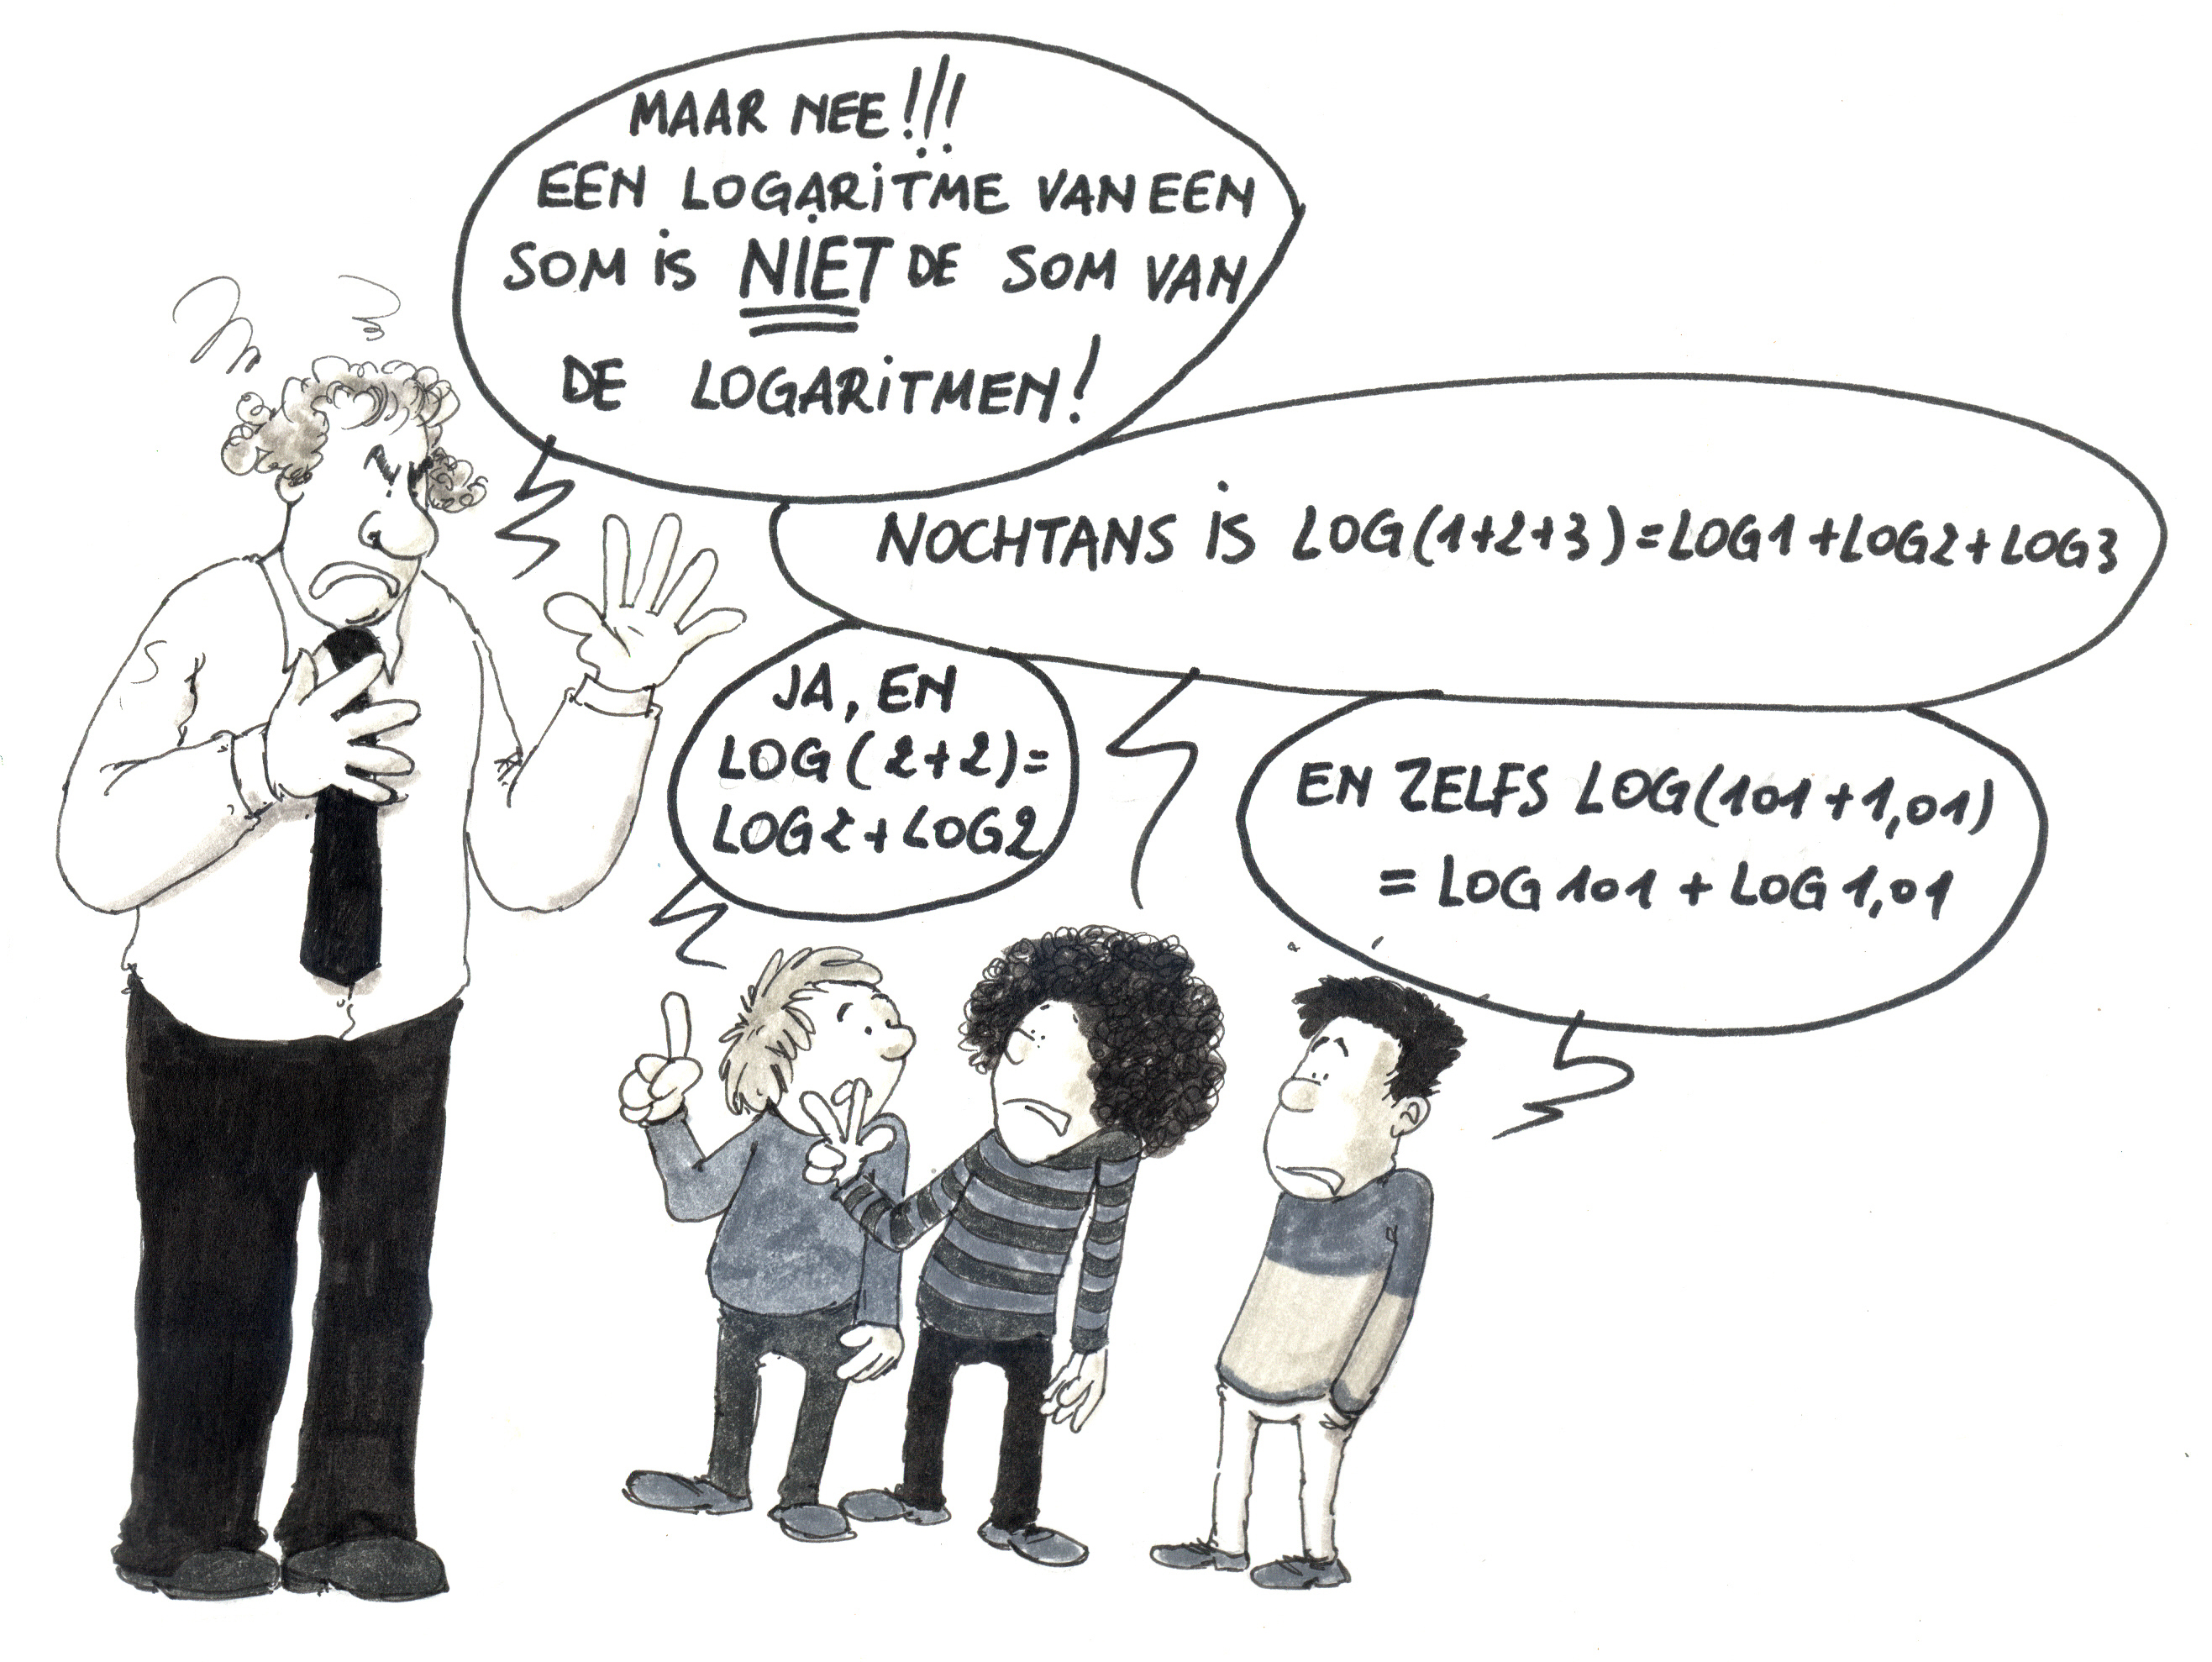
\includegraphics[width=0.75\linewidth]{img/logsom.jpg}
\end{center}
\begin{multicols}{2}

De oorsprong van logaritmen is het omzetten van een vermenigvuldiging in een optelling. In de 16de eeuw schreef de Duitse monnik en wiskundige Michael Stifel de tabel op van figuur \ref{tabelstifel} (Stifel, 1544). De bovenste rij is een rekenkundige rij en de onderste een meetkundige. Hij schreef erbij in het Latijn (de wetenschappelijke taal van die tijd):
\begin{quote}
\emph{Qualiacunque facit progressio geometrica multiplicando et dividendo, tali facit progressio arithmetica addendo et subtrahendo.}
\end{quote}
(Alles wat de meetkundige rij doet door te vermenigvuldigen en te delen, hetzelfde doet de rekenkundige rij door op te tellen en af te trekken.)
\begin{figure}[H]
\begin{center}
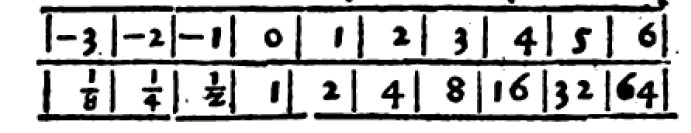
\includegraphics[width=\linewidth]{img/tabelstifel}
\captionof{figure}{Tabel uit Aritmetica Integra}
\label{tabelstifel}
\end{center}
\end{figure}

Bijvoorbeeld om $\frac{1}{8}\cdot 32$ te berekenen, kun je de getallen die erboven staan optellen: $-3+5=2$. Het product $\frac{1}{8}\cdot 32$ is dan het getal dat onder $2$ staat, namelijk $4$. De lezer herkent de rekenregel: de logaritme van een product is de som van de logaritmen. Immers, door van de onderste naar de bovenste rij te gaan, neem je $\log_2$, de logaritme met grondtal $2$. Door logaritmen op te tellen, vind je de logaritme van het product:
$$-3+5 = {}\log_2\frac{1}{8} + {}\log_2 32 = \log_2\left(\frac{1}{8}\cdot 32\right).$$
Ditzelfde idee, het koppelen van een rekenkundige en een meetkundige rij, maar dan zonder negatieve getallen en breuken, ontstond al vele eeuwen vroeger bij de Babyloniërs (18de eeuw v.C., zie miniwerktekst hieronder) en kwam ook voor bij Archimedes (3de eeuw v.C.).

\end{multicols}

\beginwerktekst{Een Babylonische kleitablet}

Een kleitablet bevat de volgende tabel:
\begin{center}
\begin{tabular} {| c | c |}
\hline
2 & 1\\
4 & 2\\
8 & 3\\
16 & 4\\
32 & 5 \\
64 & 6\\
\hline
\end{tabular}
\end{center}
We weten niet of die gebruikt werd om het vermenigvuldigen van de getallen uit de eerste kolom te vergemakkelijken. Misschien wilden de makers van het kleitablet enkel de machten van $2$ nummeren. Maar er is ook een kleitablet teruggevonden met de volgende tabel. Hier gaat het alvast niet over nummeren.

\begin{center}
\begin{tabular} {| c | c |}
\hline
2 & 15\\
4 & 30\\
8 & 45\\
16 & 1\\
\hline
\end{tabular}
\end{center}

\begin{enumerate}
    \item Wat had je eerder verwacht dan die 1 in de laatste rij? Waarom staat er een 1?
    
\emph{Je verwacht $60$. Maar Babyloniërs rekenden in het zestigtallig talstelsel: $60$ (eenheden) is $1$ (zestigtal). Uit de context moest je afleiden of een $1$ de betekenis had van $1$ of van $60$ of van $60^2$ of... Er was immers geen teken voor $0$.}

\item Kun je dit bekijken als een tabel van een logaritmische functie? Zo ja, wat is hier het grondtal?

\emph{Ja. Het grondtal is $\sqrt[15]{2}$.}
\end{enumerate}


\eindewerktekst

\begin{multicols}{2}
 
Rond het jaar 1000 had een Arabische sterrenkundige, Ibn-Yunus, ook een manier bedacht om een product om te zetten in een som. Hij steunde op wat we nu zouden noteren als de formule $\cos a\cdot \cos b=\frac {1}{2} \left( \cos(a+b)+\cos(a-b) \right)$, niet zo eenvoudig dus.
\tussentitel{Logaritmetabellen}
Na Stifel was er nog een weg te gaan om te komen tot een tabel die een handige rekenhulp vormt. Het is niet moeilijk om de tabel van figuur \ref{tabelstifel} naar links en naar rechts uit te breiden, maar je wilt natuurlijk ook andere getallen vermenigvuldigen of delen dan enkel machten van $2$. De grote gaten tussen de machten van $2$ moesten nog worden opgevuld.

In de 17de eeuw groeide de nood aan precieze berekeningen, onder meer met de sterrenkunde van de Deen Tycho Brahe en de Duitser Johannes Kepler. Het idee van Stifel werd door de Schot John Napier en de Engelsman Henri Brigg geperfectioneerd.

Napier werkte twintig jaar aan een tabel die een meetkundige rij met heel kleine tussenstapjes omzet in een rekenkundige rij. Hij kon altijd tussenstapjes toevoegen omdat hij aan een continu proces dacht: een punt beweegt op een rechte zodat het evenveel tijd nodig heeft voor een interval $[1, r]$ als voor $[r, r^2]$, als voor $[r^2,r^3]$, enz. Meer hierover vind je in Clark en Montelle, 2011.

Het woord logaritme is van Napier. Het betekent aantal verhoudingen (van het Grieks $\lambda\rm o\gamma\rm o\varsigma$ verhouding en $\alpha\rho\iota\theta\mu\rm o \varsigma$ getal, aantal). Napier schreef:
\begin{quote}
\emph{Logarithmi sunt numeri qui proportionalibus adjuncti aequales servant differentias.}
\end {quote}
(Logaritmen zijn getallen die verwijzen naar gelijke verhoudingen en die gelijke verschillen hebben.)

Dank zij Brigg werd als grondtal voor de tabellen $10$ genomen, wat veel handiger is in ons tiendelig talstelsel. Op die manier ontstonden tabellen zoals die tot ongeveer 1980 op school werden gebruikt!

In de volgende werktekst maken de leerlingen kennis met het gebruik van logaritmetabellen. We gebruiken hier niet de oorspronkelijke tabellen van Napier en Brigg, maar die van Schons en De Cock (z.d.), die wij nog op school hebben gebruikt. Merk op: het gebruik van logaritmetabellen gaat sneller dan het cijferen, enkel wanneer je het gewoon bent. Leerlingen die de eerste keer met dergelijke tabellen geconfronteerd worden, zullen het wellicht een hele klus vinden. Het is ook niet de bedoeling dat ze hier handig in worden, maar enkel dat ze kennis maken met het principe ervan.

\end{multicols}




\beginwerktekst{Berekeningen met logaritmetabellen}

We willen een vermenigvuldiging uitvoeren aan de hand van logaritmen, om minder te moeten cijferen. We gaan ervan uit dat we niet over een rekenmachine beschikken (anders zouden we die vermenigvuldiging gewoon intypen). We beschikken wel over logaritmetabellen. Omdat jullie waarschijnlijk geen tabellenboekje op de bank hebben liggen, zullen in deze werktekst de nodige stukken van de tabel voorzien zijn.

Als eerste voorbeeld nemen we $7603\cdot 75,53$. We bepalen dit product stap voor stap met logaritmetafels. Wellicht ga je vinden dat dit een hele klus is, maar voor wie de logaritmetafels gewoon was, ging het toch sneller dan gewoon het product te becijferen...

Eerst zoeken we $\log 7603 = \log_{10} 7603$ op. Hier is het betreffende stuk van de tabel.



\begin{werktekstoef}
\item Wat lees je af bij $7603$?

\emph{In de rij van $760$ en de kolom van $3$ zien we $098$ maar daar moet nog $88$ voor, dat een beetje hoger staat. Dus: $88098$.}

\item Kan dit wel de 10-logaritme zijn van $7603$?

\emph{Neen, omdat $7603$ tussen $1000$ en $10000$ ligt, moet $\log 7603$ een getal zijn tussen $3$ en $4$.}

\begin{figure}[H]
\begin{center}
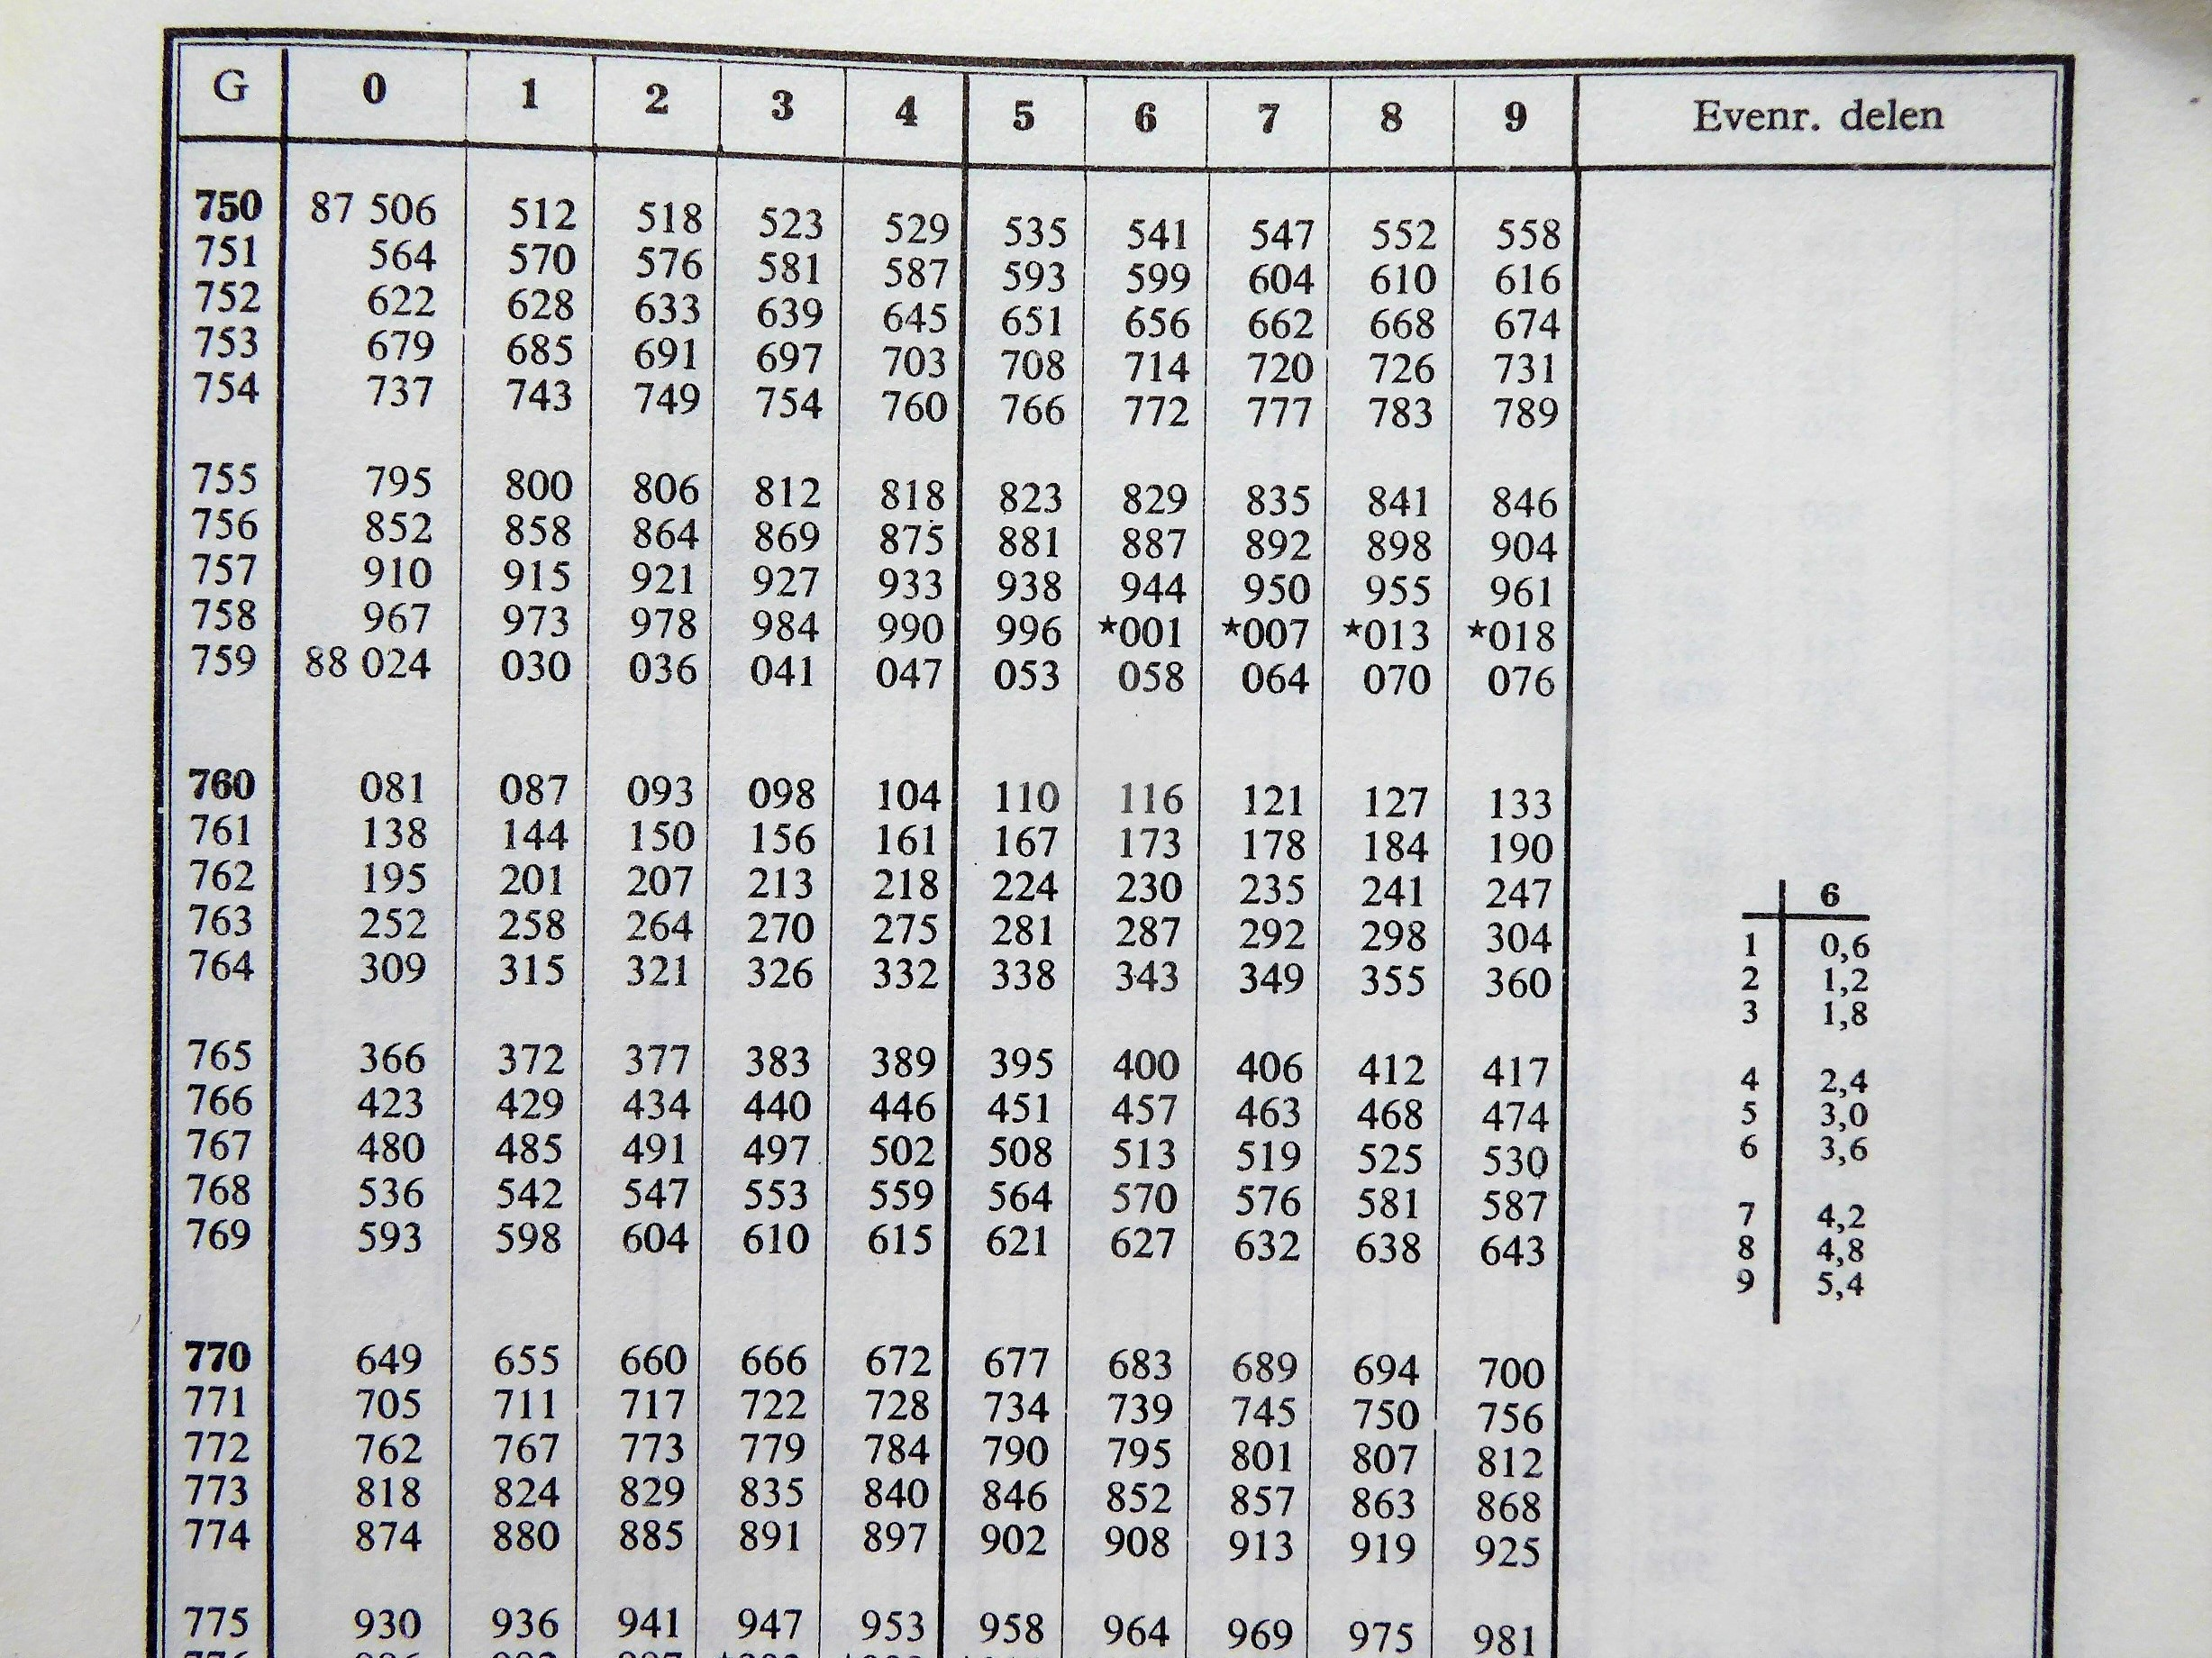
\includegraphics[width=0.9\linewidth]{img/schonsp19}

\end{center}
\end{figure}
\end{werktekstoef}

De cijfers voor de komma van de logaritme vormen de \emph{wijzer} en de cijfers na de komma de \emph{mantisse}. De tabel geeft enkel de mantisse; de wijzer moet je uit het hoofd bepalen. In de inleiding van het tabellenboekje lezen we hierover het volgende, onder de titel `ter herinnering' (immers: voor de leerlingen uit de tijd van de tabellenboekjes was dit niet nieuw):

\begin{quote}
\emph{De wijzer van de logaritme van een getal groter dan $1$ is één minder dan het aantal cijfers in de gehelen van dat getal} [...]. \emph{Wordt een getal vermenigvuldigd met (of gedeeld door) $10^n$, dan wordt de mantisse van zijn logaritme niet gewijzigd, maar de wijzer telt $n$ eenheden meer (of minder). In de tabel staan de mantissen van de logaritmen der getallen van $1000$ tot $10000$.}

\end{quote}

\begin{werktekstoef}

\setcounter{enumi}{2}

\item Wat is nu $\log 7603$?

\emph{De wijzer is $3$ en de mantisse is wat we daarnet opzochten, $88098$. Dus: $\log 7603=3,88098$.}

\item Bepaal (met, toevallig, hetzelfde stukje tabel) $\log 75,53$.

\emph{We zoeken de mantisse op van $\log 7553$. We vinden $87812$. De wijzer is nu $1$ want het getal ligt tussen $10$ en $100$. (Of: volgens het citaat uit de inleiding: $1$ minder dan het aantal cijfers in de gehelen, dus $1$ minder dan $2$.) Besluit: $\log 75,53=1,87812$.}

\end{werktekstoef}

Nu we de twee logaritmen hebben, kunnen we het product zoeken.

\begin{werktekstoef}

\setcounter{enumi}{4}

\item Leg uit: $\log \left(7603\cdot 75,53\right)=5,75910$.

\emph{De logaritme van het product is de som van de logaritmen. De som van de twee logaritmen die we gevonden hebben, is inderdaad (cijferen!) $5,75910$.}

\item Waarom zijn we er nog niet?

\emph{We kennen nu de logaritme van het product; we moeten het product zelf nog zoeken.}

\end{werktekstoef}

Om terug te zoeken van welk getal $5,75910$ de logaritme is, moet je opnieuw een onderscheid maken tussen de wijzer $5$ en de mantisse $75910$. Voor deze laatste gebruik je dit stukje tabel.



\begin{werktekstoef}
\setcounter{enumi}{6}
\item Wat weet je door de wijzer?

\emph{Het product is een getal tussen $10^5$ en $10^6$.}

\item Vind je de mantisse terug in de tabel? Zo niet, tussen welke twee getallen zitten we?

\emph{We vinden $75906$ en $75914$ als mantissen in de tabel. $75910$ zit in het midden. $75906$ is de logaritme van $5742$ en $75914$ is de logaritme van $5743$. Rekening houdend met de wijzer, moet het product dat we zoeken  dus ergens tussen $574 200$ en $574 300$ liggen. Dit is zo omdat $\log$ een stijgende functie is. Maar de grafiek van $\log$ is niet recht; dus zal het niet exact $574 250$ zijn.}

\item In de tijd van de tabellenboekjes was het de gewoonte om `lineair te interpoleren', dit wil zeggen om te doen alsof de grafiek tussen de punten van de tabel, recht is. Wat zou dit hier geven voor het gezochte product? 

\emph{Dit zou geven: $7603\cdot 75,53\approx574 250$.}

\item Vergelijk met het echte product (nu even wel met de rekenmachine).

\emph{Het echte product is $574254,59$.}
\begin{figure}[H]
\begin{center}
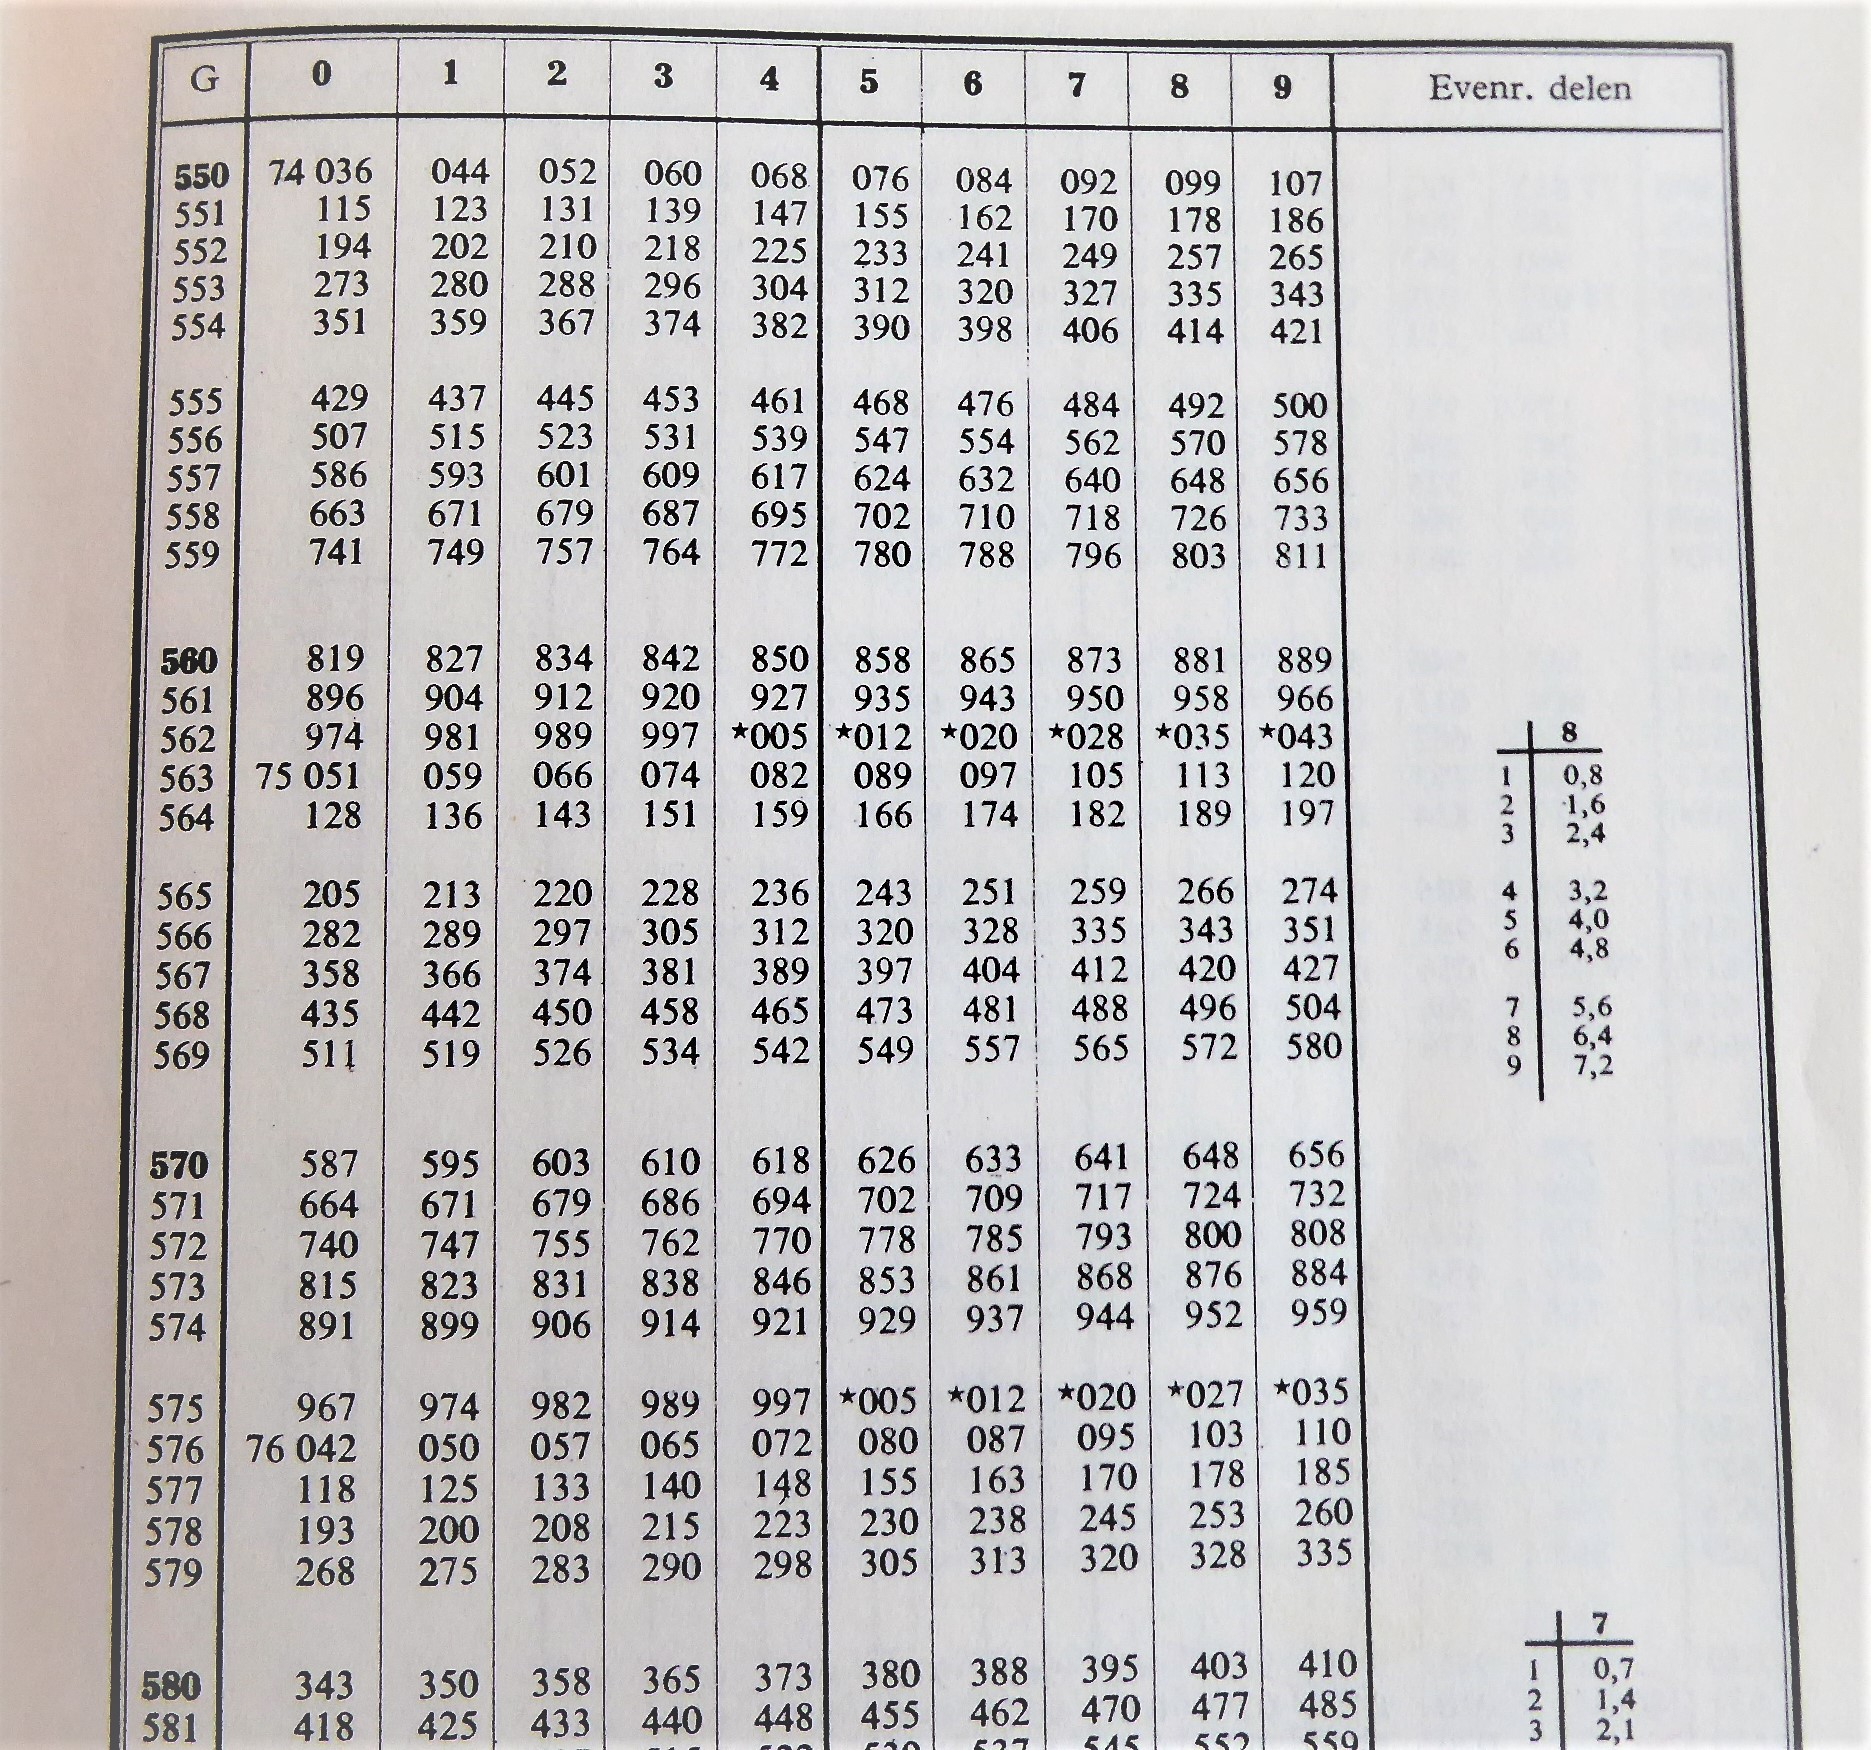
\includegraphics[width=0.90\linewidth]{img/schonsp15}
\end{center}
\end{figure}
\end{werktekstoef}

\eindewerktekst

\begin{multicols}{2}
 Uiteraard kun je met de leerlingen, na deze stap-voor-stap-opdracht, een oefening maken waarbij de leerlingen iets gelijkaardigs doen zonder deelvraagjes. Ook een deling (door de logaritmes af te trekken) kan aan bod komen. We willen wel benadrukken dat het helemaal niet de bedoeling is dat de leerlingen het werken met logaritmetabellen aanleren en inoefenen. Het is enkel de bedoeling om het te begrijpen en te ervaren, en om op die manier in te zien hoe gemakkelijk het toch wel geworden is met onze rekenmachines. We hebben in de werktekst het lineair interpoleren niet uitgebreid besproken. Toevallig was het hier niet nodig omdat we knal in het midden zaten. Eerder dan het leren lineair interpoleren (al dan niet door gebruik te maken van de tabelletjes `evenredige delen' die je misschien in de rechterkolom van de logaritmetabellen hebt opgemerkt), vinden we het interessanter dat ze (grafisch) inzien waarom dat interpoleren maar een benadering is.
 
 De volgende werktekst, geïnspireerd door Daems (2019), bevat een aantrekkelijk fragment uit De Decker, 1626. Leerlingen die wel eens te creatief zijn met spelling, zullen zich hier goed bij voelen...
\end{multicols}

\beginwerktekst{Een rechthoekige driehoek uit 1626}

\begin{figure}[H]
\begin{center}
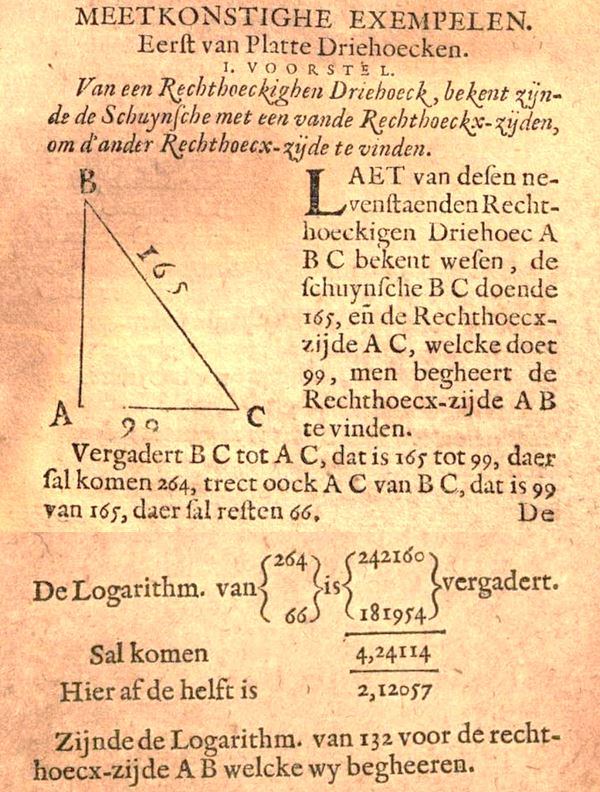
\includegraphics[width=0.65\linewidth]{img/pythmetlog}

\end{center}
\end{figure}

\begin{werktekstoef}
\item Lees het eerste deel van de tekst (tot en met de tekst naast de tekening). Wat is de opgave?

\emph{Van een rechthoekige driehoek waarvan de schuine zijde en een rechthoekszijde gegeven zijn, de tweede rechthoekszijde zoeken.}

\item Met welke berekening zou je deze oefening oplossen?

\emph{$|AB|=\sqrt{165^2-99^2}=132$.}

\item{Hoe wordt dit in de tekst berekend?}

\emph{Men neemt eerst de som en het verschil van de gegeven afmetingen:$|BC|+|AC|=165+99=264$; $|BC|-|AC|=165-99=66$.}

\emph{Hiervan neemt men de logaritmen (waarbij de komma wordt weggelaten, maar dit wordt verderop hersteld). Deze logaritmen worden opgeteld (`vergaderd') en van deze som neemt men de helft. Ten slotte zoekt men op waarvan dit de logaritme is:}

$$\frac{1}{2} \left( \log (165+99)+\log(165-99)\right)=\log{??}\Rightarrow ??=132.$$

\item Waarom klopt het?

\emph{$\frac{1}{2} \left( \log (165+99)+\log(165-99)\right)=\frac{1}{2}\log\left((165+99)(165-99)\right)=\frac{1}{2} \log(165^2-99^2)=\log\sqrt{165^2-99^2}.$}

\emph{Bij de eerste en de derde gelijkheid steunden we op eigenschappen van logaritmen; bij de tweede op het merkwaardig product `product van toegevoegde tweetermen'.}

\emph{En $\log\sqrt{165^2-99^2}$ is inderdaad de $\log$ van de gezochte zijde (zie de hedendaagse berekening in vraag 2).}



\end{werktekstoef}
\eindewerktekst

\begin{multicols}{2}

Het volledige boek waaruit dit voorbeeld komt, staat online (zie Decker, 1626). Wie gaat kijken, zal merken dat er nog meer parels van voorbeelden in staan. Leerlingen die zin hebben in meer, kunnen er hun gading vinden. Maar alweer willen we benadrukken dat het niet de bedoeling is om dit in te oefenen... We willen vooral laten zien hoe logaritmen gebruikt werden toen vermenigvuldigingen, delingen, worteltrekkingen... nog niet met een druk op een knop tevoorschijn kwamen.

\tussentitel{Hoe zelf een stukje van een logaritmetabel maken?}

Laten we zoeken naar benaderingen voor $\log1$, $\log2$, $\log3, \ldots \log10$ zonder rekenmachines of andere hulpmiddelen te gebruiken. We beperken ons hier tot ruwe benaderingen; voor bruikbare tabellen zijn natuurlijk betere benaderingen nodig en steunt men bijvoorbeeld op reeksontwikkelingen. We baseren ons hier op Resnikoff en Wells (1973).

$\log 1 =0$

Voor $\log 2$ vertrekken we van een macht van $2$ waarvan we bij benadering de $\log_{10}$ kunnen bepalen omdat deze macht van $2$ ongeveer gelijk is aan een macht van $10$:

$2^{10}=1024\approx 1000=10^3$

$\Rightarrow\log 2^{10} \approx \log 10^3$

$\Rightarrow 10 \log 2\approx 3 \log 10 = 3$

$\Rightarrow \log 2\approx 0,30$

Voor $\log 3$ doen we iets gelijkaardigs, steunend op $\log 2$ die we al benaderd hebben:


$3^9=19683\approx 2\cdot 10^4$

$\Rightarrow 9 \log 3 \approx \log 2 + 4$

$\Rightarrow \log 3 \approx \frac{1}{9} (0,30 + 4)\approx 0,48$

Voor $\log 7$:

$7^2=49\approx 50=\frac{10^2}{2}$

$\Rightarrow \log 7\approx \frac {1}{2}(\log 10^2-\log 2)\approx \frac{1}{2}(2-0,30)\approx 0,85$

Voor $\log 4$ gebruiken we $4=2^2$; voor $\log 6$ gebruiken we $6=2\cdot 3$; voor $\log 8$ steunen we op $8=2^3$ en voor $\log 9$ op $9=3^2$.


\subsection{Rekenlinialen}
Naast logaritmetabellen werden rekenlinialen uitgevonden door de Britse wiskundigen Edmud Gunther en William Oughtred, eveneens in de 17de eeuw. Het principe is eigenlijk hetzelfde: het omzetten van een vermenigvuldiging (deling) in een optelling (aftrekking). Optellen en aftrekken gebeurt hier niet door te cijferen maar door lijnstukken achter elkaar te plaatsen. Later werden nog allerlei schalen toegevoegd om er ook andere dingen mee te kunnen berekenen. Tot ongeveer 1980 was de rekenliniaal een dagelijks hulpmiddel voor ingenieurs. Merk op dat de astronauten die in 1969 naar de maan vlogen, een rekenliniaal op zak hadden! Dit is te zien op foto's van toen (figuur \ref{astronauten1}).
\begin{figure}[H]
\begin{center}
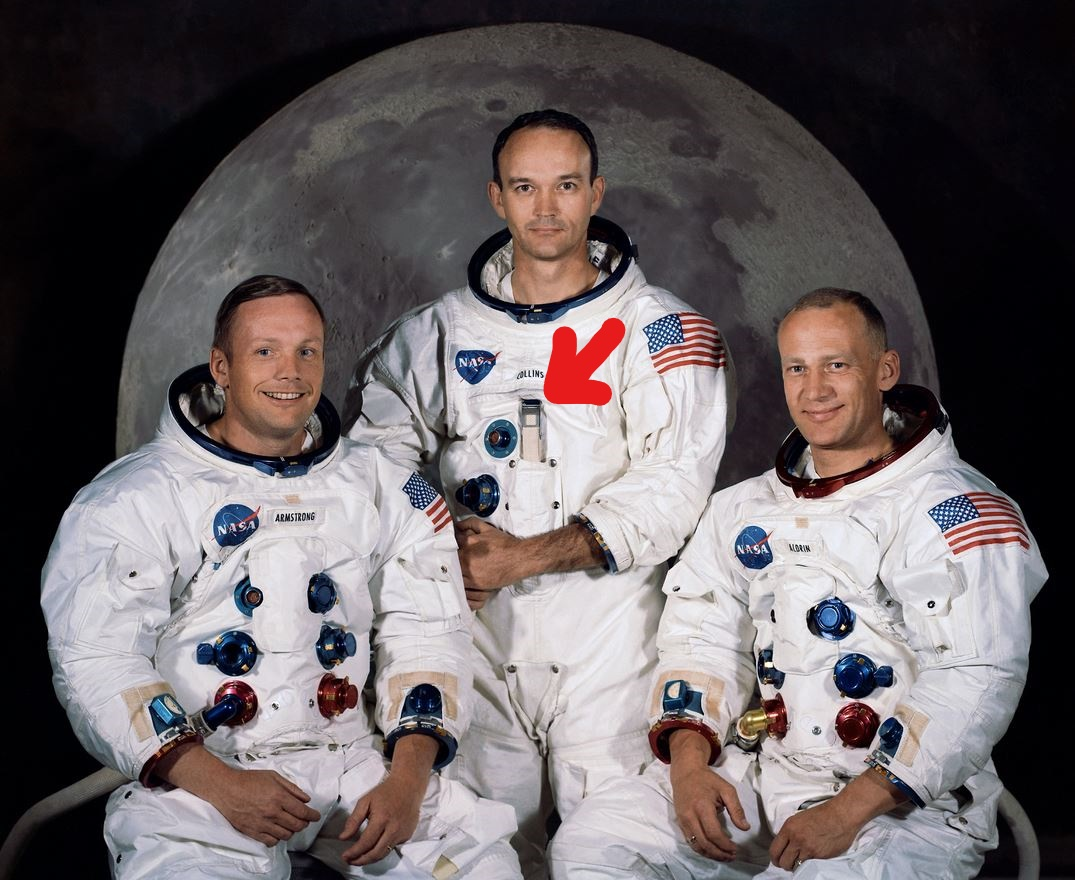
\includegraphics[width=1\linewidth]{img/astronauten1}
\captionof{figure}{Neil Armstrong, Mike Collins and Buzz Aldrin in 1969, met rekenliniaal}
\label{astronauten1}
\end{center}
\end{figure}
In de eerste werktekst hieronder ontdekken leerlingen dit principe met zelfgemaakte logaritmische schalen. We werken met heel eenvoudige vermenigvuldigingen en delingen om te focussen op het principe zonder complicaties. We negeren hierbij de andere schalen die op echte rekenlinialen voorkomen.

Vooraf kun je de leerlingen voorbereiden op het principe van een rekenliniaal, door twee getallen te laten optellen met twee (gewone) latten of geodriehoeken tegen elkaar. Om $4+6$ te berekenen, leg je bijvoorbeeld de $4$ van de lat tegen de $0$ van de geodriehoek, en ga je kijken bij welk getal van de lat de $6$ van de geodriehoek ligt (figuur \ref{geo}). Het zal je niet verbazen dat dit $10$ is.
\begin{figure}[H]
\begin{center}
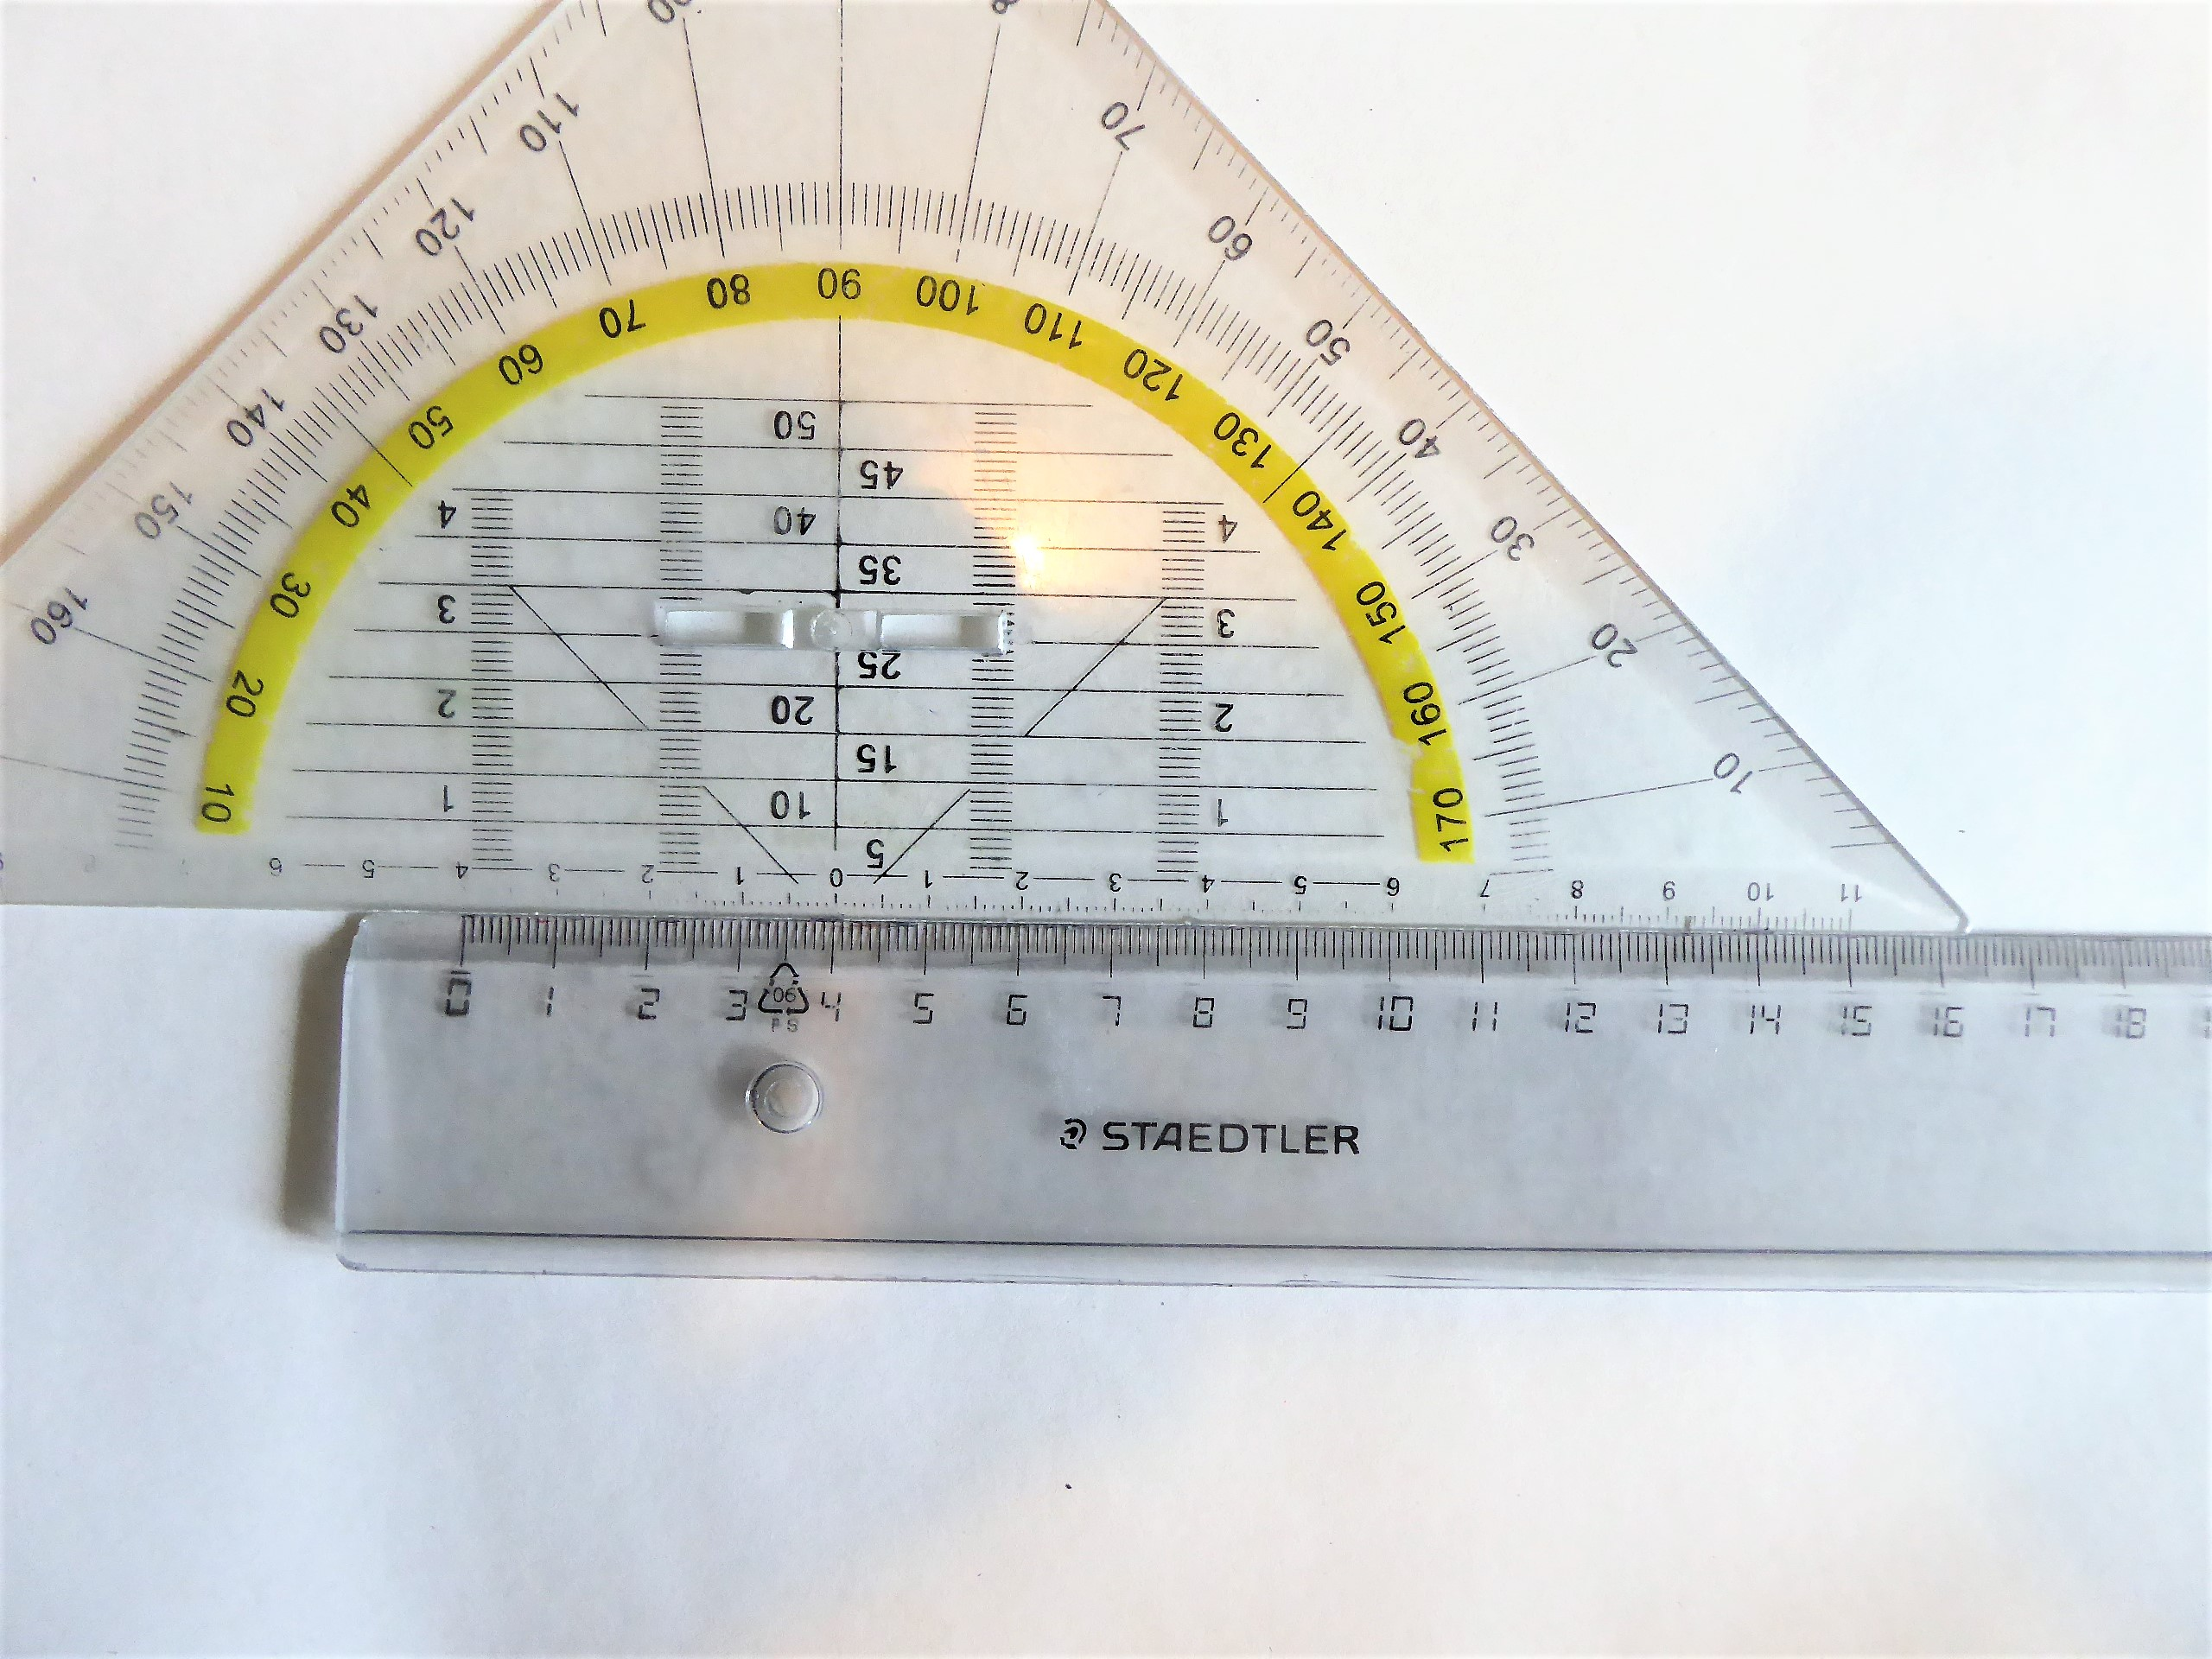
\includegraphics[width=1\linewidth]{img/geo}
\captionof{figure}{Optellen met een lat en een geodriehoek}
\label{geo}
\end{center}
\end{figure}
\end{multicols}

\vspace{3cm}
\begin{center}
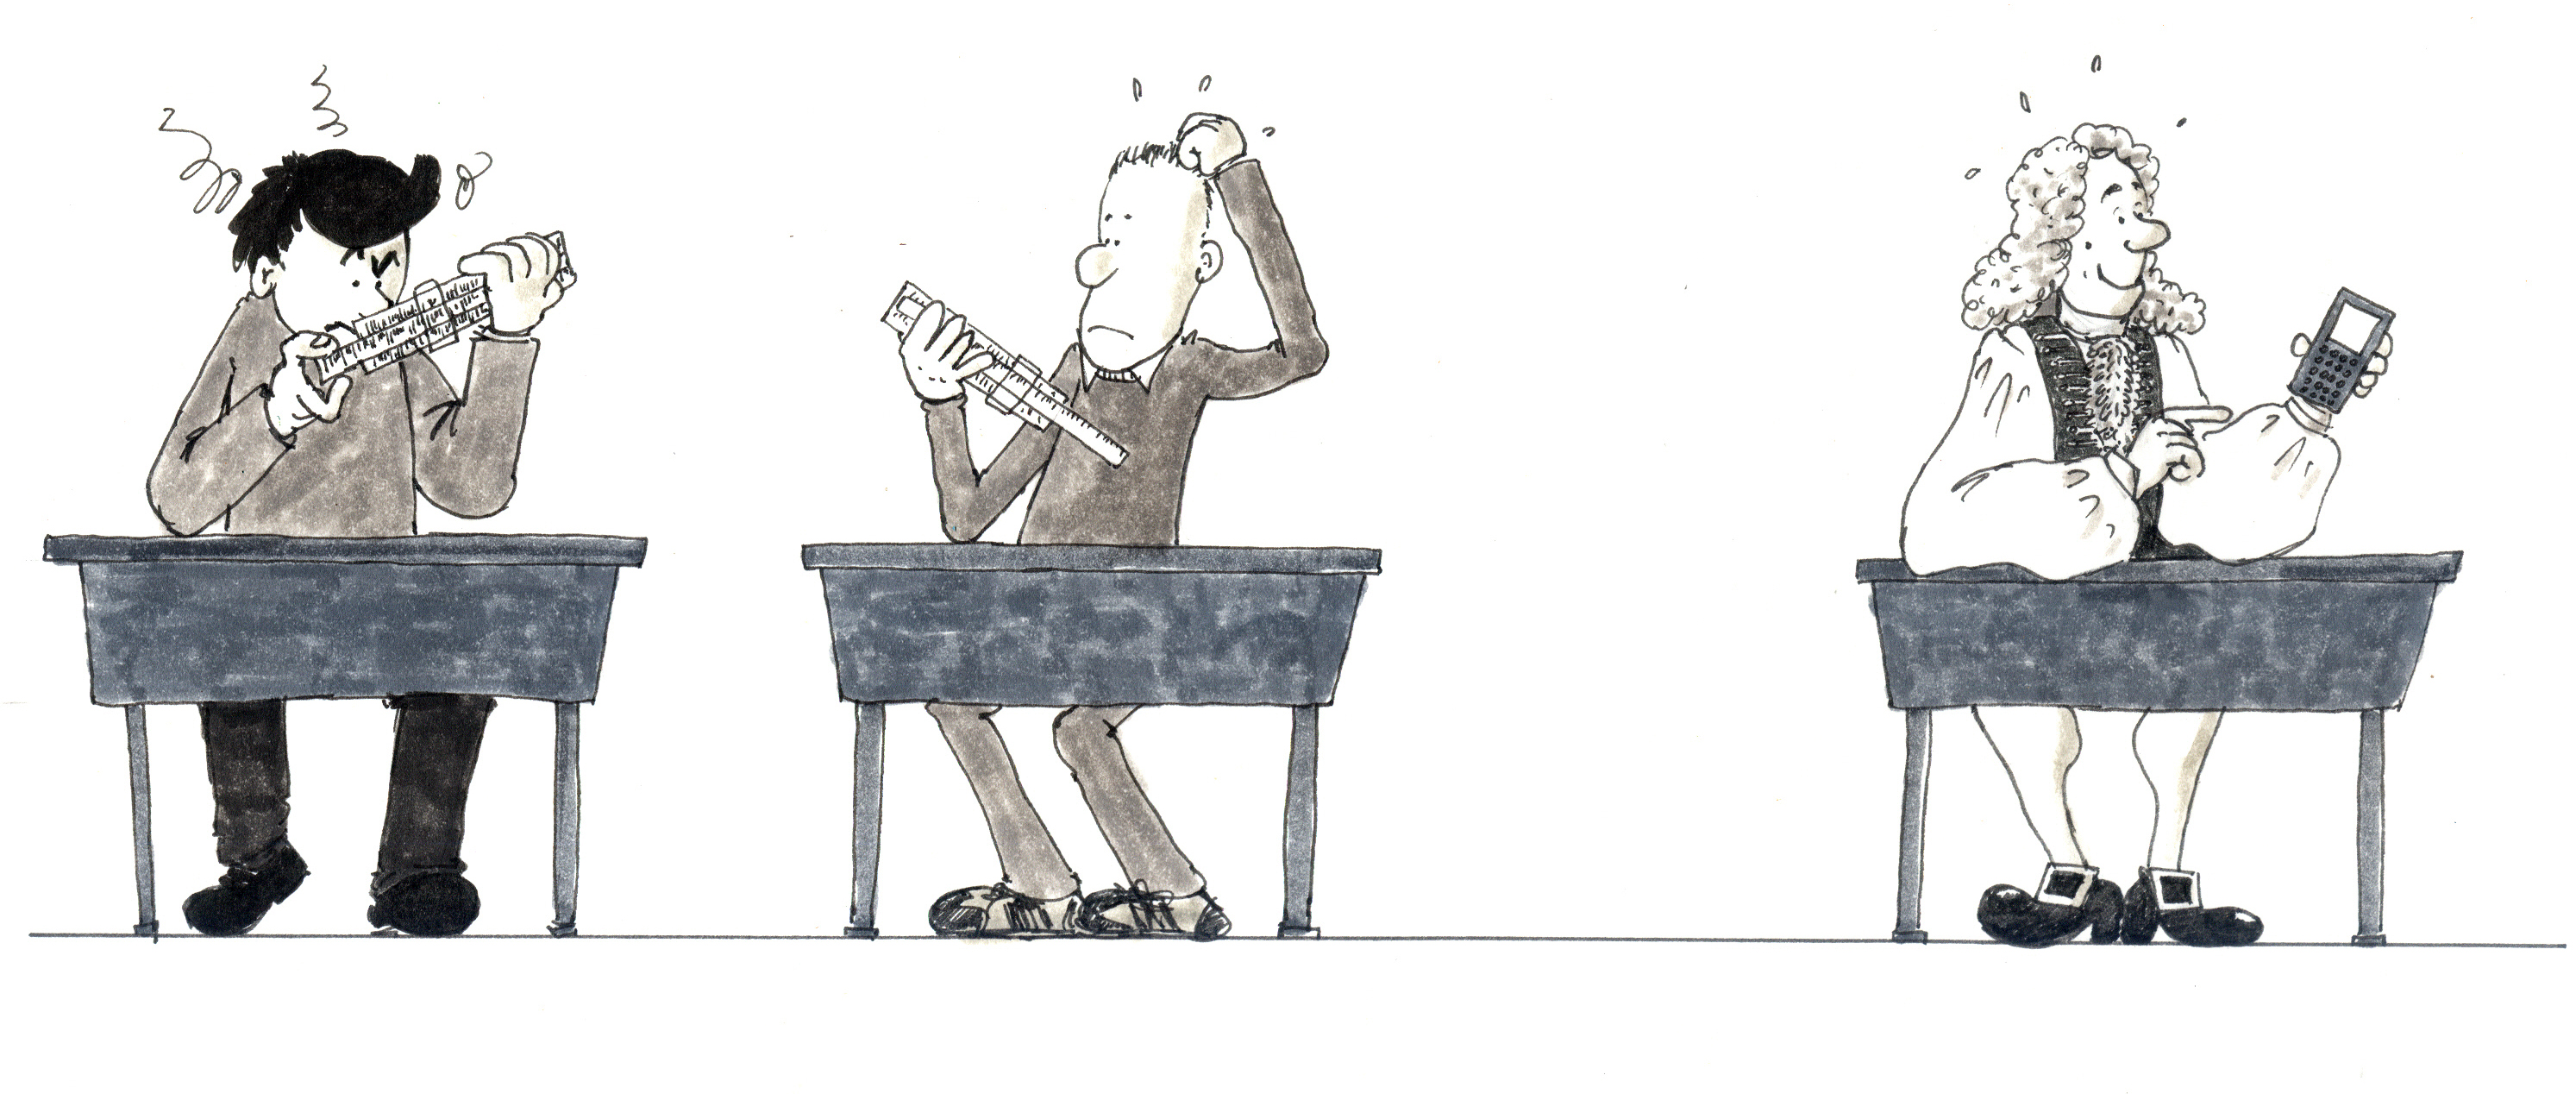
\includegraphics[width=1\linewidth]{img/rekenlat.jpg}
\end{center}
\begin{multicols}{2}\newpage
\end{multicols}

\newpage

\beginwerktekst{Logaritmische schalen en een eenvoudige rekenliniaal}

\tussentitel{Een logaritmische schaal}

Hetzelfde principe als bij de logaritmetabellen, namelijk het omzetten van een vermenigvuldiging (deling) in een optelling (aftrekking) via logaritmen, is ook de basis van de rekenliniaal. Heb je een oma of opa die wetenschappelijke studies heeft gedaan, dan zal die zeker vaak een rekenliniaal gebruikt hebben.

In een eerste stap werken we  met eenvoudige berekeningen die je meteen uit het hoofd kunt maken, zoals $2\cdot 3$. De rekenliniaal is hiervoor natuurlijk niet nuttig, maar hiermee willen we de werkwijze verduidelijken. We maken hiervoor een vereenvoudigde rekenliniaal, bestaande uit twee latjes voorzien van logaritmische schalen. Nadien maken we een paar oefeningen met een `echte' rekenliniaal.

Om een logaritmische schaal te maken, plaatsen we de getallen $1, 2, 3, \ldots, 10, 20, 30, \ldots, 100$ op een getallenas, niet op de gewone manier, even ver van elkaar, maar zodanig dat de afstand van elk getal $n$ tot het getal $1$ gelijk is aan $\log n$.

\begin{figure}[H]
\begin{center}
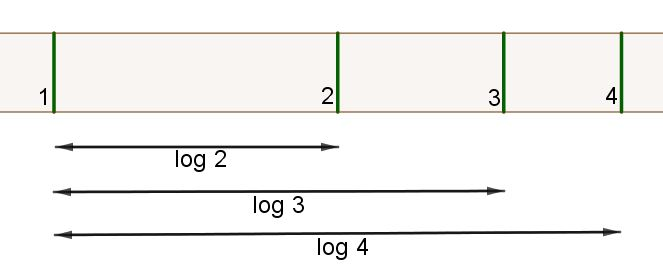
\includegraphics[width=0.55\linewidth]{img/startlogschaal}

\end{center}
\end{figure}

\begin{werktekstoef}
\item Waar is $0$ op deze schaal?

\emph{Oneindig ver aan de linkerkant, want $\log 0 = -\infty$.}

\item Ligt $1,5$ op de logaritmische schaal in het midden tussen $1$ en $2$?

\emph{Neen, dichter bij $2$ dan bij $1$, want $\log 1,5 = 0,176\dots$}

\item Teken twee latjes met logaritmische schalen voor de getallen $1, 2, 3, \ldots, 10, 20, 30, \ldots, 100$, met als lengte-eenheid $1$ dm (tussen $1$ en $10$ dus). Knip ze uit.

\emph{Zoiets moet het worden.}

\begin{figure}[H]
\begin{center}
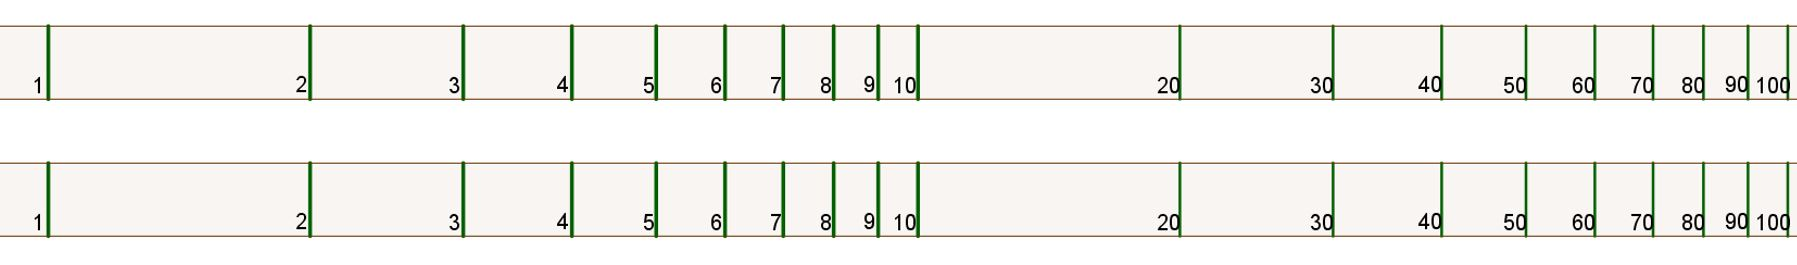
\includegraphics[width=0.95\linewidth]{img/logschalen}

\end{center}
\end{figure}

\item Als je die schaal aan beide kanten zou verlengen, wat kun je zeggen over de plaats van de getallen $0,01$; $0,1$; $1$; $10$; $100$; $1000\ldots$?

\emph{Die liggen even ver van elkaar, namelijk $1$ eenheid.}

\end{werktekstoef}

\tussentitel{Een eenvoudige vermenigvuldiging en deling}

\begin{werktekstoef}

\setcounter {enumi}{4}

\item We weten wel dat je $2\cdot 3$ uit het hoofd kent. Maar hoe zou je dit product kunnen bepalen met deze logaritmische schalen?

\emph{We tellen $\log 2$ en $\log 3$ op door het lijnstuk tussen $1$ en $2$ op het bovenste latje (lengte $\log 2$) en het lijnstuk tussen $1$ en $3$ op het onderste latje (lengte $\log 3$) achter elkaar te plaatsen. De totale lengte van $1$ op het bovenste latje tot $3$ op het onderste latje heeft dan als lengte $\log 2 + \log 3 = \log (2\cdot 3)$. Het getal op het bovenste latje boven de $3$ van het onderste latje geeft dus het product. En, jawel, het is $6$.}

\begin{figure}[H]
\begin{center}
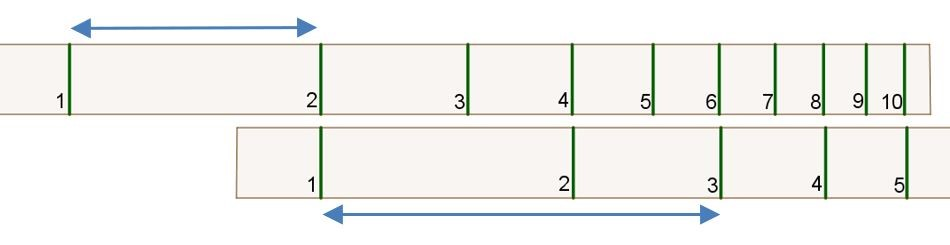
\includegraphics[width=0.65\linewidth]{img/tweemaaldrie}

\end{center}
\end{figure}

\item Laat zien hoe je met deze latjes de deling $30 : 5$ kunt bepalen.

\emph{Van de lengte tussen $1$ en $30$ op het bovenste latje trekken we de lengte tussen $1$ en $5$ op het onderste latje af. Dit doen we door de $5$ onder de $30$ te plaatsen. Boven de $1$ van het onderste latje lezen we het quotiënt af: het is $6$.}

\begin{figure}[H]
\begin{center}
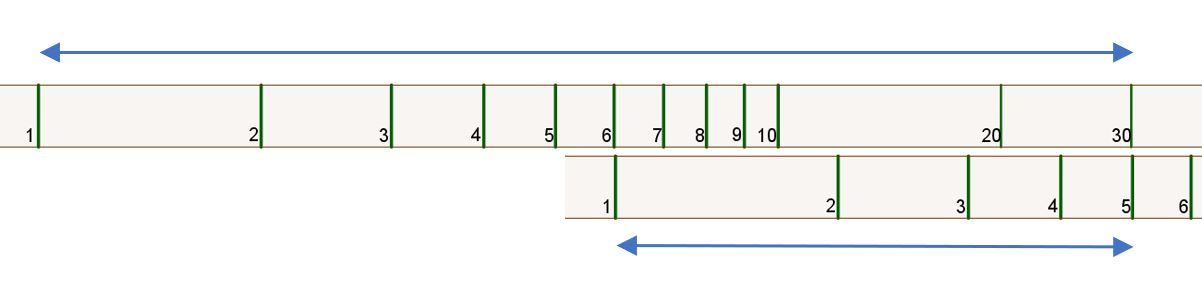
\includegraphics[width=0.85\linewidth]{img/dertiggedeelddoorvijf}

\end{center}
\end{figure}

\end{werktekstoef}

\tussentitel{Wat als de latjes te kort zijn?}

Voor $6\cdot 50$ zijn onze latjes te kort. En toch gaat het, bijvoorbeeld zo: in plaats van de $1$ plaatsen we de $10$ van het onderste latje onder de $6$. Wat we boven $50$ aflezen, namelijk $30$, is dan een tiende van de uitkomst. Dus: $6 \cdot 50 = 30\cdot 10=300.$

\begin{figure}[H]
\begin{center}
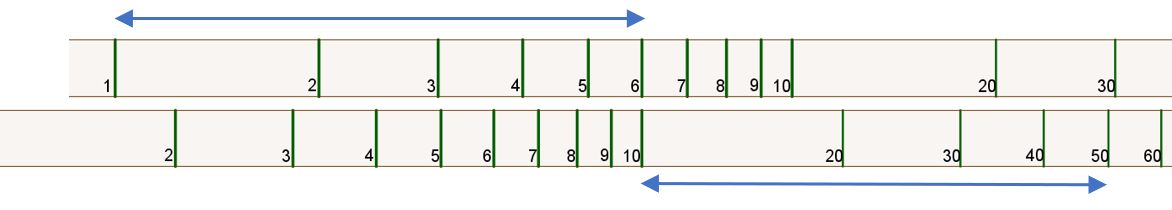
\includegraphics[width=0.90\linewidth]{img/zesmaalvijftig}

\end{center}
\end{figure}

\begin{werktekstoef}

\setcounter {enumi}{6}

\item Verklaar waarom dit werkt.

\emph{Bij het lijnstuk met lengte $\log 6$ is de lengte tussen de merkstrepen $10$ en $50$ bijgeteld. De lengte die men bepaalt is dus $\log 6 + (\log 50 - \log 10)$. Dit is gelijk aan $\log 6\cdot \frac{50}{10}$, dus inderdaad de $\log$ van een tiende van wat we zochten.}

\end{werktekstoef}

Dus: als de latten te kort zijn, dan gebruikt men in plaats van de $1$ een andere macht van $10$ en passen we op het einde aan door de komma te verplaatsen. In het geval van ons simpel latje is die macht van $10$ gewoon $10$ zelf. 

\begin{werktekstoef}

\setcounter {enumi}{7}

\item Leg uit hoe je $3:5$ kunt bepalen met onze simpele rekenliniaal.

\emph{Zoals bij de vorige deling, plaatsen we deler $5$ onder het deeltal $3$. Boven de $1$ zouden we de uitkomst moeten aflezen, maar ons bovenste latje is niet lang genoeg aan de linkerkant. Dus lezen we af wat er boven de $10$ staat ($6$). Dit is tien keer de uitkomst die we zoeken; we moeten nog delen door $10$. Dus: $3:5=0,6$.}

\begin{figure}[H]
\begin{center}
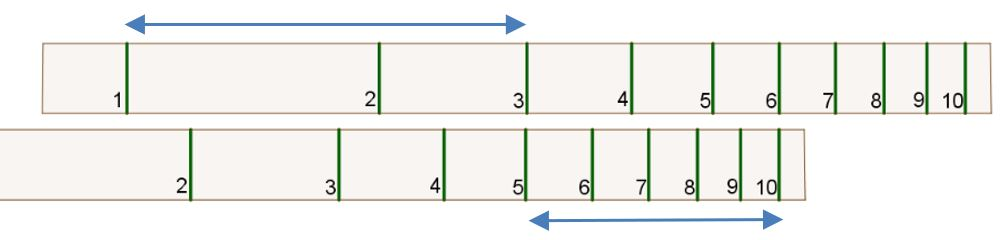
\includegraphics[width=0.75\linewidth]{img/driegedeelddoorvijf}

\end{center}
\end{figure}

\emph{Verklaring: we telden eigenlijk het stuk tussen $5$ en $10$ (lengte: $\log 10 -\log 5$) op bij de lengte $\log 3$. We verkregen dus een lengte van $\log 3 + \log 10 - \log 5$ en dat is $\log (\frac {3}{5}\cdot 10)$, dus de $\log$ van tien keer wat we zochten.}

\end{werktekstoef}
\eindewerktekst


\begin{multicols}{2}
Uiteraard diende de rekenliniaal niet om berekeningen zoals $2\cdot 3$ uit te voeren. In een volgende fase werken de leerlingen met echte rekenlinialen (als je hierover beschikt) of met uitgeknipte, zie static.scientificamerican.com (volledige url zie bronnen), of met een app uit Wolf (2019). 

Je kunt leerlingen bijvoorbeeld laten berekenen hoeveel $2,75\cdot 3,18$ is. In figuren \ref{aristo1} en \ref{aristo2} hebben we dit berekend met de app Aristo Junior van Wolf (2019) en lezen we als antwoord $8,75$ af, een benadering voor het echte product $8,745$. We gebruikten enkel de C- en de D-lijn met `gewone' logaritmische schalen. Als de afdruk hieronder te klein is, gebruik de app!

\end{multicols}
\begin{center}

\begin{figure}[H]

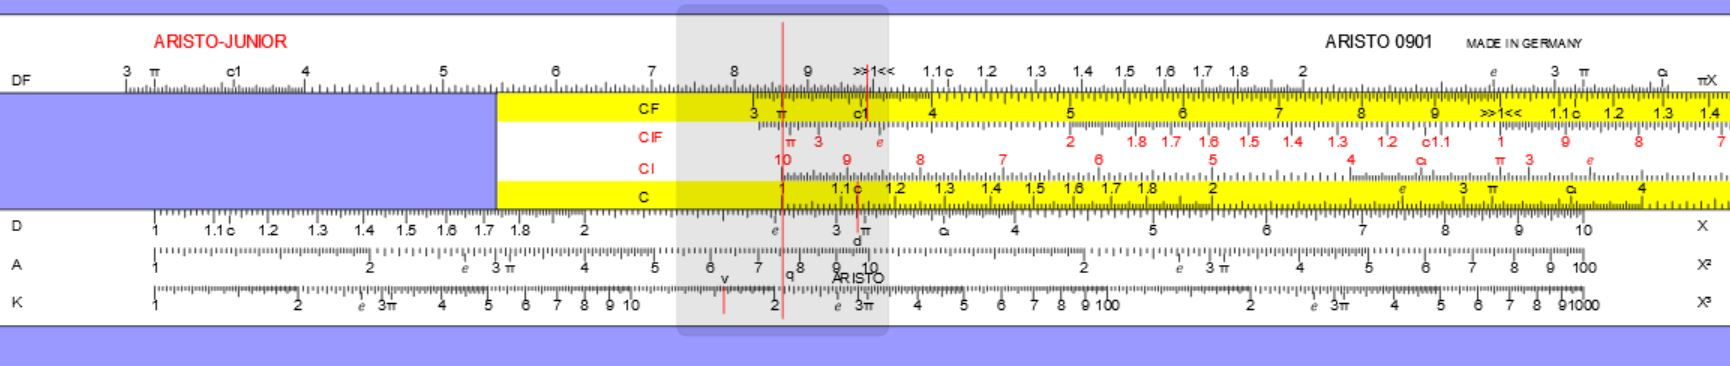
\includegraphics[width=\linewidth]{img/aristo1}
\captionof{figure}{$2,75\cdot 3,18$: cursorlijn op $2,75$ van de D-lijn en hierop de $1$ van de C-lijn verschuiven}
\label{aristo1}
\end{figure}

\begin{figure}[H]

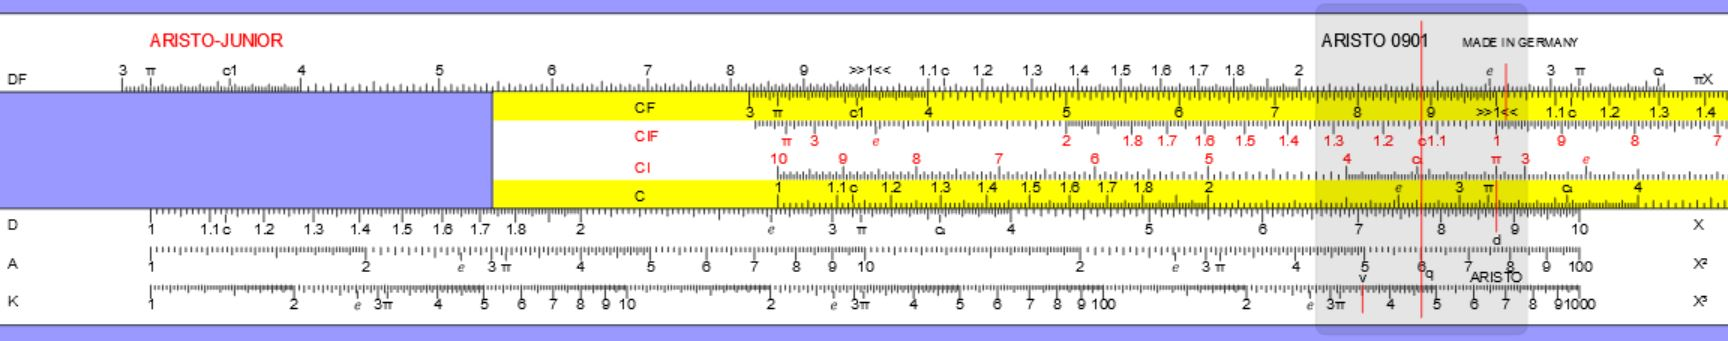
\includegraphics[width=\linewidth]{img/aristo2}
\captionof{figure}{$2,75\cdot 3,18$: cursorlijn naar $3,18$ van de C-lijn verschuiven en resultaat aflezen op de D-lijn: $8,75$ ongeveer}
\label{aristo2}
\end{figure}

\begin{figure}[H]

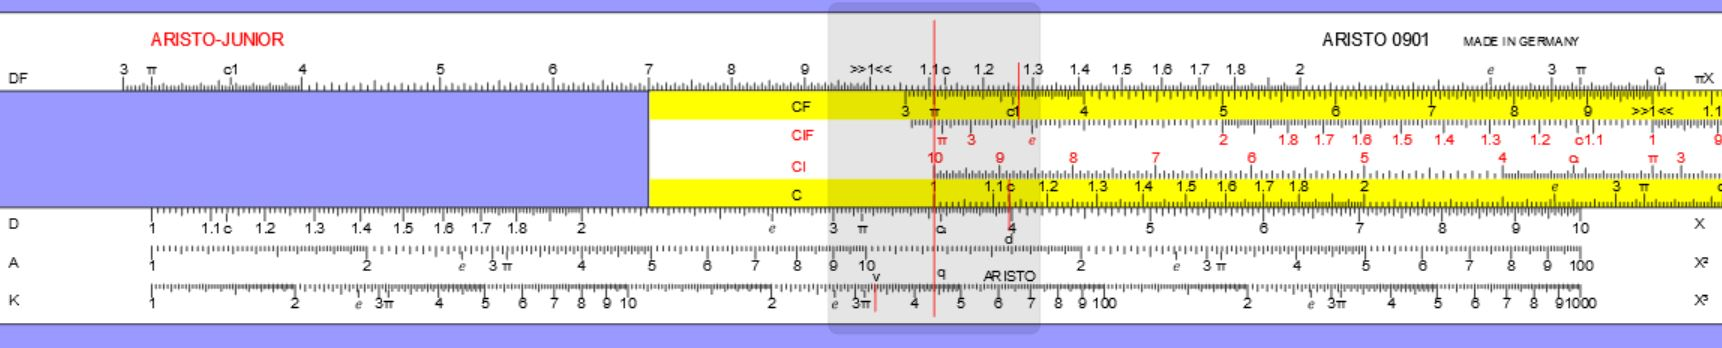
\includegraphics[width=\linewidth]{img/aristo3}
\captionof{figure}{$35,3\cdot 188$: cursorlijn op $3,53$ van de D-lijn en hierop de $1$ van de C-lijn verschuiven}
\label{aristo3}
\end{figure}

\begin{figure}[H]
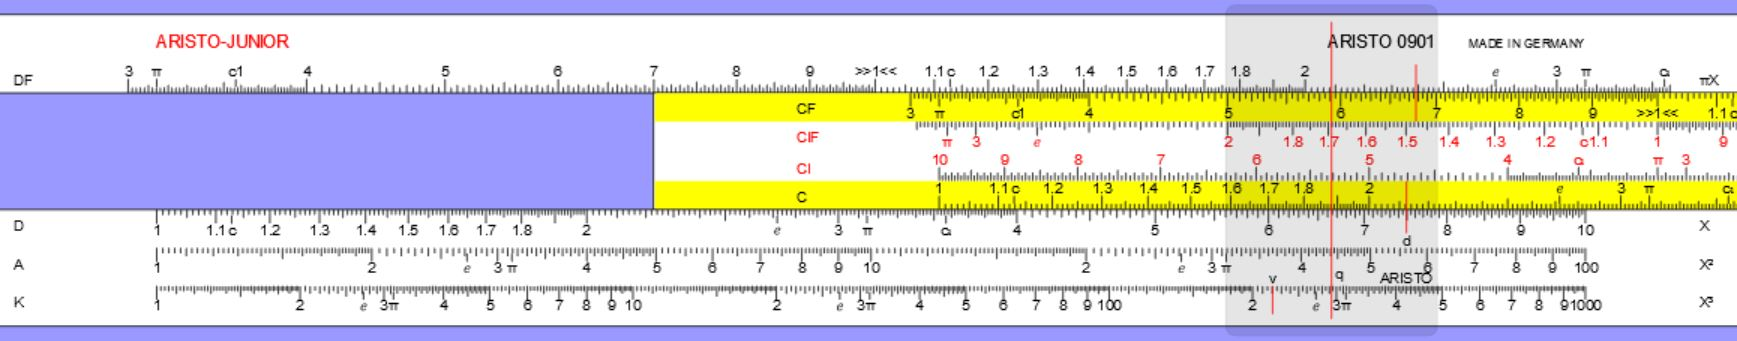
\includegraphics[width=\linewidth]{img/aristo4}
\captionof{figure}{$35,3\cdot 188$: cursorlijn naar $1,88$ van de C-lijn verschuiven en resultaat aflezen op de D-lijn: $6,65$ ongeveer, nog te vermenigvuldigen met de juiste macht van $10$}
\label{aristo4}
\end{figure}
\end{center}
\begin{multicols}{2}
In de figuren \ref{aristo3} en \ref{aristo4} wordt $35,3\cdot 188$ berekend. Met de rekenliniaal wordt afgelezen dat $3,53\cdot 1,88$ ongeveer gelijk is aan $6,65$. De komma moet nog drie plaatsen naar rechts geschoven worden. Dit geeft $6650$, als benadering voor het product $6636,4$. 

Laat de leerlingen voor elkaar één of twee opgaven verzinnen, vermenigvuldigingen of delingen. Om binnen het beschikbare interval van de rekenliniaal te blijven, moet er desnoods gewerkt worden op een factor $10^k$ na, en nadien aanpassen. Wie liever nog enkele opgaven met oplossing heeft, kan die vinden in van Poelje (2014), handout 3.

De echte rekenlinialen, en ook de app-versies, bevatten nog andere schalen dan de twee logaritmische schalen die dienen om te vermenigvuldigen en te delen. We gaan hier niet op in, maar nieuwsgierige leerlingen kunnen dit natuurlijk altijd uitzoeken... 

Toch nogmaals benadrukken dat ons doel niet is de leerlingen te trainen in het werken met tabellenboekjes en rekenlinialen!

\subsection{Verdere evoluties in de geschiedenis van logaritmen}

In de loop van de 17de eeuw ontstond de analytische meetkunde. Krommen werden beschreven met algebraïsche vergelijkingen. De Vlaamse jezuïet Gregorius van Sint-Vincent en de Nederlander Christiaan Huygens vonden op een meetkundige manier een verband tussen oppervlakte onder de hyperbool $xy=1$ en logaritmen. Later werd dit verband met integralen geformuleerd ($\int_1^x \frac{1}{t} \text d t = \ln x$).

Met de Zwitser Leonhard Euler (18de eeuw) werden logaritmen gezien als `exponenten' bij het grondtal. Dit is de manier waarop wij nu meestal de logaritmen invoeren. Ook in de 18de eeuw werden logaritmen uitgebreid tot complexe getallen, maar daar gaan we niet op in.

\section{Toepassingen van logaritmen}

\subsection{Aantal cijfers van het grootste gekende priemgetal}

We starten met een kleine (maar fijne) toepassing in verband met grote priemgetallen. In deze werktekst verklappen we niet te veel. We hopen dat (sommige) leerlingen op het idee komen om rekenregels te gebruiken om een logaritme te berekenen die buiten het bereik ligt van de rekenmachine. Uiteraard kun je als leraar meer tips geven aan leerlingen die dat nodig hebben.

\end{multicols}

\beginwerktekst{Het grootste priemgetal?}

Het grootste priemgetal bestaat niet, want er zijn oneindig veel priemgetallen. Euclides (3de eeuw v.C.) bewees dat elke eindige lijst priemgetallen onvolledig is.

Maar: er is wel iets als het grootste ‘gekende’ priemgetal. Op dit moment (juni 2019) is dat het Mersennegetal $2^{82589933}-1$. 

Een Mersennegetal is $1$ minder dan een macht van $2$. In de 17de eeuw bestudeerde Marin Mersenne priemgetallen van die vorm. Niet alle getallen van die vorm zijn priemgetallen en soms zat Mersenne er naast: hij dacht bv. dat $2^{67}-1$ priem is, maar later bleek dat dit getal gelijk is aan $193707721\cdot 761838257287$. Bij de zoektocht naar grote priemgetallen werkt men nog steeds heel vaak met Mersennegetallen, want voor die getallen bestaat er een efficiëntere manier om de deelbaarheid te controleren (de Lucas-Lehmertest, zie Eggermont en Vanlommel, 2012).

\begin{werktekstoef}

\item Kun je dit grootste gekende priemgetal met je rekenmachine berekenen?

\emph{Je krijgt ‘overflow’. De grootste macht van $2$ die mijn TI-84+ (van 2010) kan berekenen (of liever:in wetenschappelijke notatie kan omzetten) is $2^{332}$.}

\item Hoeveel cijfers heeft dit getal? Tip: gebruik logaritmen.

\emph{Het aantal cijfers van een getal (dat geen macht van $10$ is) is de afronding naar boven van de $10$-log van dat getal. Bv. getallen van drie cijfers liggen in het interval $[100, 1000[$, zodat hun 10-logaritme gelegen is in $[\log{100},  \log{1000}[=[2, 3[.$}

\emph{Maar: ook $\log(2^{82589933}-1)$ kan de rekenmachine niet berekenen. Met de rekenregels gaat het wel (bij benadering):}

$$\log(2^{82589933}-1)\approx\log(2^{82589933})= 82589933 \log 2\approx 24862047,17.$$

\emph{Besluit: het grootste priemgetal (in juni 2019) heeft $24862048$ cijfers.}

\item Als je dit priemgetal uitschrijft op een lange strook papier, met een klein lettertype van \'e\'en cijfer per mm, hoelang is de strook dan?

\emph{Bijna 25 km.}

\end{werktekstoef}
\eindewerktekst

\begin{multicols}{2}


\subsection{Zintuigen werken logaritmisch}
De Duitse arts Ernst Heinrich Weber (1795-1878) publiceerde in 1834 zijn onderzoek over de tastzin van de huid en het gehoor. Daarin formuleerde hij een wet die de samenhang tussen prikkeling (stimulus) en waarneming (sensatie)  weergeeft.

Eén van zijn experimenten ging als volgt: de hand van een (geblinddoekte) proefpersoon ligt op een tafel. Op deze hand wordt een massa gelegd. De zwaartekracht van deze massa veroorzaakt een prikkeling die de proefpersoon gewaarwordt als een druk. Als men een bijkomende massa op de hand legt, dan vergroot de prikkel maar de proefpersoon zal dit niet altijd merken. Het verschil in prikkel moet groot genoeg zijn om het te kunnen waarnemen. Er is dus een onderscheid tussen de prikkel en het waarnemen. De prikkel komt binnen via zintuigen (huid, ogen, neus, oren, ogen) en wordt naar de hersenen geleid. Deze prikkel wordt bijvoorbeeld omgezet in pijn, beeld, stank of geluid. Pas als dit gebeurt kunnen we spreken van een waarneming of sensatie.

Een belangrijk aspect van dit onderzoek is de absolute drempel van een prikkel of stimulus. Hierbij wordt gemeten bij welk niveau een stimulus opgemerkt wordt. Het kan hierbij bijvoorbeeld gaan om het zwakste licht dat door een oog gedetecteerd wordt, het zwakste geluid dat gehoord wordt door een oor of de lichtste aanraking van de huid die gevoeld wordt. Bij een zeer laag niveau zal het licht, het geluid, de aanraking nooit opgemerkt worden, bij een hoog niveau altijd. Men gebruikt een uitgebreid panel van gezonde proefpersonen om die drempelwaarden experimenteel vast te leggen. De gemiddelde mens ziet, hoort, ruikt, voelt... vanaf deze drempelwaarden.

Naast deze drempelwaarde wordt de differentiële drempel onderscheiden. De differentiële drempel geeft aan wat het kleinste verschil is tussen twee stimuli om het verschil op te merken.  We stellen de waarneming (in het Duits: Empfindung) voor door $E$  en de prikkel (in het Duits: Reiz) door $R$.  Weber stelde dat voor een even grote toename in waarneming $\Delta E$ er een relatieve prikkelstijging $\frac{\Delta R}{R}$ nodig is. Weber stelde dat de verandering in waarneming recht evenredig is met de relatieve prikkelverandering.  In formulevorm
\[\Delta E\sim \frac{\Delta R}{R}\]
met $E$ de waarneming en $R$ de prikkel.

Later zal de Duitse psycholoog en filosoof Gustav Theodor Fechner (1801-1887) dit verder wiskundig uitwerken. Het verband dat Fechner ontdekte is later bekend geworden als de wet van Weber-Fechner en is als volgt te omschrijven:

\[\frac{d E}{d R}= k \cdot\frac{1}{R}.\]
Bijgevolg moet $E$ als functie van $R$ op een constante term na logaritmisch verlopen.
\[E=k\cdot \ln R+C.\]
Als we  $R_0$ de grootste net niet waarneembare prikkel noemen, dan is $E(R_0)$ de ondergrens die we kunnen waarnemen.
\[0=k\cdot \ln R_0+C\Rightarrow C=-k \cdot \ln R_0\]
En dan is 
\[E=k\cdot \ln R -k \cdot \ln R_0\]
wat we kunnen herschrijven als
\[E=k\cdot (\ln R - \ln R_0)=k\cdot\ln \frac{R}{R_0}.\]
Als de prikkel groot is ten opzichte van de drempelwaarde, is $\frac{R}{R_0}\gg1.$
Voor grote waarden stijgt de $\ln $-functie zeer traag. Dus voor zulke prikkels stijgt de gewaarwording nauwelijks, ook als de prikkel sterk toeneemt.
De waarneming $E$ wordt een meetbare grootheid eens men $R_0$ vastgelegd heeft. De keuze van $k$ legt de eenheid van $E$ vast.

Door de rekenregel van verandering van grondtal, kun je ook overgaan op een logaritme met een ander grondtal.
\[E=k\cdot\ln \frac{R}{R_0}=k\cdot\frac{\log_b \frac{R}{R_0}}{\log_b e}.\]
Omdat elk grondtal $b$ mogelijk is, kun je $k$ gelijk stellen aan $\log_b e$ en dan wordt de formule heel eenvoudig:
\[E=\log_b \frac{R}{R_0}.\]
De sensatie is een logaritme van de relatieve prikkel.



\tussentitel{Geluid en decibels}
In de praktijk zal men de waarneming $E$ aanvullen met een eenheid om te laten zien dat het een meetbare grootheid is. Zo komt men bij het meten van het geluidsniveau tot de eenheid `bel'(B) als het grondtal van de logaritme 10 is en de prikkel 10 keer de geluidsdrempel is.
\[E(10R_0)=\log \frac{10R_0}{R_0}=\log 10=1 \textrm{bel}.\]
De `decibel'(dB) is dan een $ 10^{\textrm{de}}$ hiervan.
Deze eenheid wordt vooral gebruikt in de akoestiek. De prikkel is in dit geval de geluidsintensiteit $I$, de waarneming de geluidssterkte of het geluidsniveau.
\[E(I)=10\cdot\log \frac{I}{I_0}\textrm{dB}.\]
We gaan hier verder op in in de werktekst.

Geluidsmetingen zijn almaar belangrijker geworden. Mensen zijn misschien onverdraagzamer geworden, er zijn wettelijke normen voor lawaai dat snelwegen, vliegtuigen, windmolens, fuiven, zwembaden... mogen veroorzaken, er zijn normen voor geluid op het werk. Afhankelijk van het geluidsniveau mag je langer of minder lang blootgesteld worden aan geluid om gezond te blijven.
Hieronder geven we enkele opgaven over rekenen met decibels, uit het leven gegrepen.

Op je smartphone kun je met de zoekterm geluidsmeter of decibelmeter een gratis app installeren om de geluidssterkte in dB te meten. De advertenties moet je er dan even bij nemen! Deze metingen zijn niet  geijkt omdat de apps op veel verschillende smartphones moeten werken. De calibratie kun je doen door een echte decibelmeter uit de fysicaklas te lenen of door gebruik te maken van de decibelschaal en de app ongeveer juist te ijken. Voor de toepassingen hieronder is de juiste waarde niet zo belangrijk. We willen vooral onderzoeken wat er gebeurt met het aantal dB als je de geluidsintensiteit of de afstand tot de geluidsbron verandert. Deze toepassingen bieden ook de kans om leerlingen attent te maken op het belang van verantwoord omgaan met hun oren: je hebt er maar twee en ze moeten levenslang meegaan!

\begin{figure}[H]
\begin{center}
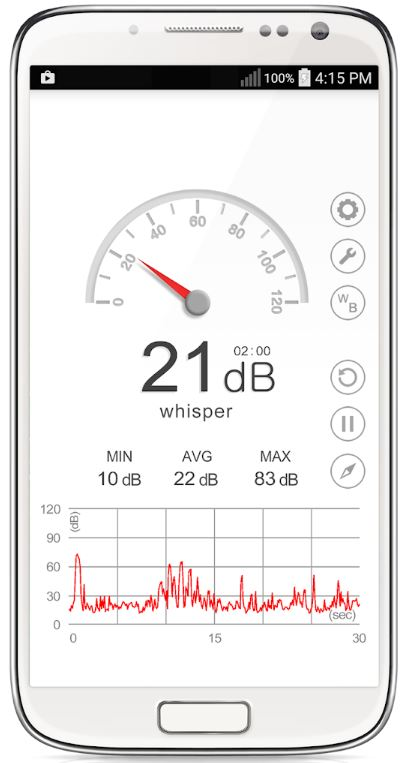
\includegraphics[width=0.45\linewidth]{img/decibelmeterapp}
\captionof{figure}{Geluidsmeter (Sound Meter) van Abc Apps}
\end{center}
\end{figure}

\end{multicols}

\beginwerktekst{Decibels}

\tussentitel{Definitie}

Een geluidsbron brengt luchtdeeltjes in trilling. Uit ervaring weten we dat dicht bij de bron (bijvoorbeeld een luidspreker) het geluid harder klinkt dan verder van de bron vandaan. Dit komt omdat de energie verdeeld wordt over een steeds groter wordend oppervlak. Hoe hard je geluid ervaart, hangt af van de geluidsintensiteit die op een bepaalde plaats heerst. De geluidsintensiteit $I$ is de hoeveelheid energie die per seconde op $1 \textrm{m}^2$ oppervlakte valt. Energie per tijdsinterval is ook gelijk aan het vermogen $P$ dus kunnen we de intensiteit $I$ ook schrijven als vermogen per oppervlakte. 
Hierbij gelden de onderstaande formules.
\[I=\frac{E}{\Delta t\cdot A}=\frac{P}{A}\]
met $I$ de intensiteit in $\frac{\textrm{W}}{\textrm{m}^2}$, $E$ de  energie in J, $\Delta t$ een tijdsinterval in s, $A$ een oppervlakte in $\textrm{m}^2$, $P$ het vermogen in W.\\
De geluidsintensiteit hangt af van het vermogen van de bron en van de afstand tot de bron. We moeten onderscheid maken tussen soorten geluidsbronnen. Bij een min of meer puntvormige geluidsbron (knippen met je vingers, een ontploffing...) zal de energie zich uitspreiden over een boloppervlak, bij een lijnvormige bron, bijvoorbeeld een drukke autoweg, zal de energie zich verspreiden volgens een cilindermantel.
\begin{figure}[H]
\begin{center}
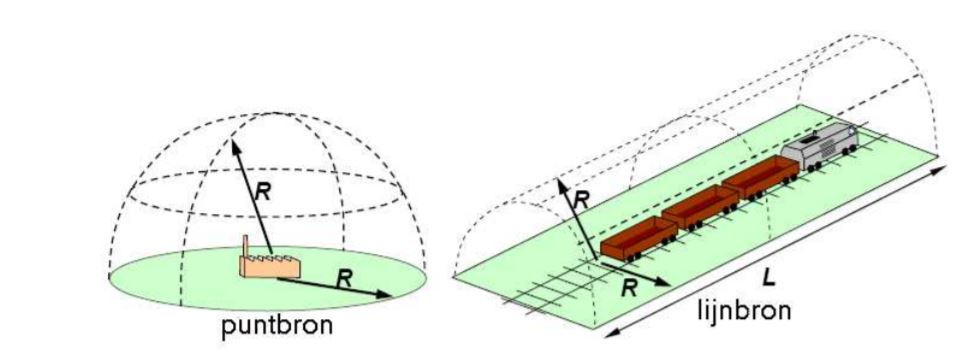
\includegraphics[width=0.90\linewidth]{img/puntbronlijnbron.jpg}
\captionof{figure}{Geluidsintensiteit op een boloppervlak en een cilindermantel}
\label{}
\end{center}
\end{figure}

\begin{werktekstoef}
\item{Een luidspreker heeft een vermogen van 3,2 W. Laat met een berekening zien dat de geluidsintensiteit op een afstand van 6,0 m
van de bron $7,1\cdot 10^{-3}\frac{\textrm{W}}{\textrm{m}^2}$ bedraagt.}

$I=\frac{3,2}{4\pi 6^2}\frac{\textrm{W}}{\textrm{m}^2}= 7,1\cdot·10^{-3}\frac{\textrm{W}}{\textrm{m}^2}$

\item{Hoe groot is de geluidsintensiteit op een twee keer zo grote afstand?}

$I=\frac{3,2}{4\pi 6^2}\frac{\textrm{W}}{\textrm{m}^2}= 7,1\cdot·10^{-3}\frac{\textrm{W}}{\textrm{m}^2}$, \emph{dus vier keer zo klein.}

 \item {De gehoordrempel is het zwakste geluid dat nog gehoord kan worden. Bij een gezond persoon bedraagt de gehoordrempel $10^{-12}\frac{\textrm{W}}{\textrm{m}^2}$.
 Bereken de maximale afstand waarop de luidspreker nog hoorbaar is.}
 
\emph{Ongeveer 505 km, onwaarschijnlijk ver!}
 
\item {Waarom zal deze afstand in de praktijk een stuk kleiner zijn?}

\emph{Het geluid wordt geabsorbeerd door allerlei obstakels.}
\end{werktekstoef}

De gehoordrempel is de laagste geluidsintensiteit die nog hoorbaar is. Ons oor is gevoeliger voor sommige frequenties dan voor andere. De frequentie is het aantal trillingen per s en wordt uitgedrukt in Hz $(=\textrm{s}^{-1})$. Hoe hoger de frequentie, hoe hoger de toon klinkt. De gehoordrempel is voor verschillende frequenties anders. Dit kun je zien in de volgende grafiek. Let op: de schaal op de as is niet gewoon!
\begin{figure}[H]
\begin{center}
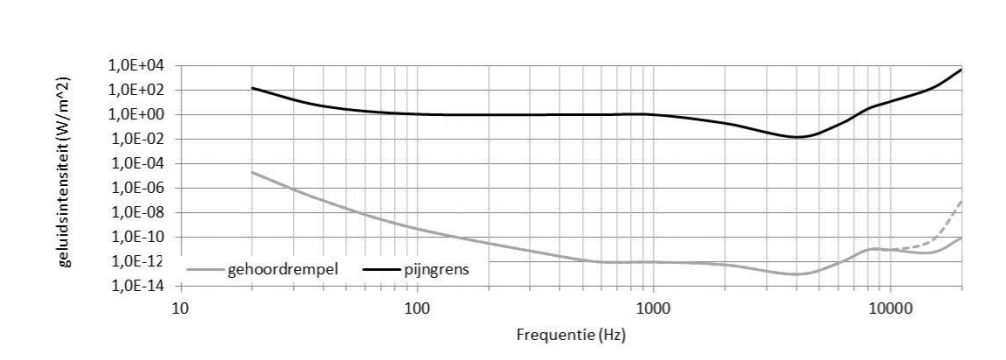
\includegraphics[width=0.85\linewidth]{img/gehoordrempel.JPG}
\captionof{figure}{Gehoordrempel en pijndrempel}
\end{center}
\end{figure}
\begin{werktekstoef}
\vspace{-1cm}
\setcounter{enumi}{4}
\item{Op de horizontale as staan de streepjes niet even ver van elkaar. Welke getallen staan er bij de streepjes tussen 10 en 100? En tussen 1000 en 10000?}

20, 30, 40,..., 90 \emph{en} 2000, 3000, 4000, ..., 9000.\

\item{ Lees uit de grafiek af bij welke frequentie ons oor het gevoeligst is.}

\emph{Bij} 4000 Hz.

\item{ Bij ouderen en mensen met gehoorbeschadiging loopt de grafiek iets anders voor frequenties boven de 10 kHz (stippellijntje). Wat merken deze personen in de praktijk van deze verandering?}

\emph{Vooral de hoge tonen zullen zij niet horen als de intensiteit niet groot genoeg is.}

\item{ Ga voor de
onderstaande geluiden na hoe we ze ervaren.
Kies uit onhoorbaar, hoorbaar, of pijnlijk/schadelijk.}

\begin{itemize}
    \item een toon van 250 Hz bij $I = 1,0\cdot10^{-10} \frac{\textrm{W}}{\textrm{m}^2}$
    \item een gesprek met frequenties tussen 250 en 4000 Hz bij $I = 1,0\cdot10^{-8} \frac{\textrm{W}}{\textrm{m}^2}$
    \item geluid van een straaljager van 2000 Hz bij $I = 2,0 \frac{\textrm{W}}{\textrm{m}^2}$
    \item een toon van 20 kHz bij $I = 1,0\cdot10^{-9} \frac{\textrm{W}}{\textrm{m}^2}$ tijdens een gehoortest voor iemand met goed gehoor.
    \item dezelfde toon voor een oudere.
\end{itemize}

\emph{Hoorbaar; hoorbaar; pijnlijk; hoorbaar; onhoorbaar.}
\end{werktekstoef}

De geluidsintensiteit $I$ is een eigenschap van de geluidsbron en heeft als eenheid $\frac{\textrm{W}}{\textrm{m}^2}$. Daarnaast wordt ook de grootheid geluidsniveau $L$ gebruikt met als eenheid de decibel (dB). Het geluidsniveau is een maat voor de waarneming van geluid. Het geluidsniveau is logaritmisch en is gedefinieerd ten opzichte van de gehoordrempel van het menselijk gehoor bij 1000 Hz ($I_0$=$10^{-12}\frac{\textrm{W}}{\textrm{m}^2}$). 

Met onderstaande formule kan het geluidsniveau in dB berekend worden:
\[L=10\cdot\log \frac{I}{I_0} \textrm{ dB}.\]

\begin{werktekstoef}
\setcounter{enumi}{8}
\item {Laat met een berekening zien dat een geluidsintensiteit van $1,0\cdot10^{-4} \frac{\textrm{W}}{\textrm{m}^2}$ overeenkomt met een geluidsniveau van 80 dB.}

$L=10 \cdot \log\frac{10^{-4}}{10^{-12}}=10 \cdot \log10^8=80$ dB.

\item {Bereken de geluidsintensiteit bij een geluidsniveau van 86 dB.}

$I=4,0\cdot10^{-4}\frac{\textrm{W}}{\textrm{m}^2}.$

\item{Bereken het geluidsniveau voor de gehoordrempel $I_0$. Kunnen er ook negatieve decibels voorkomen?}

\emph{Gehoordrempel:}0 dB. \emph{Negatieve decibels krijg je voor een geluidsintensiteit lager dan $I_0$. Dit is niet te horen door een gemiddelde mens, maar wel te meten met goede geluidsmeters! } 

\item{Een vuistregel bij het werken met decibel is dat een toename van 3 dB overeenkomt met een verdubbeling van de geluidsintensiteit en een afname van 3 dB met een halvering van de geluidsintensiteit. Ga aan de hand van de antwoorden op de vorige vragen na of dit klopt.}

\item {Meet met je smartphone hoeveel dB lawaai er is als je het zo stil mogelijk maakt in de klas. Bereken de bijbehorende intensiteit.}
\end{werktekstoef}
\begin{figure}[H]
\begin{center}
\includegraphics[width=0.90\linewidth]{img/dBtabel.png}
\captionof{figure}{Decibeltabel}
\end{center}
\end{figure}
\begin{werktekstoef}
\setcounter{enumi}{13}
\item{Probeer zoveel mogelijk lawaai te maken en meet weer het aantal dB. Bereken de bijbehorende geluidsintensiteit.}

\item{Hoeveel keer zo groot is de geluidsintensiteit uit de vorige vraag ten opzichte van de geluidsintensiteit uit de vraag daarvoor?}

\item{Probeer geluid te maken met een constant geluidsniveau. Verdubbel dit nu. Bv twee toetertjes of piepende smartphones vergelijken met één toetertje of smartphone. Meet het aantal dB voor de twee. Maakt het verschil of je dit doet met een zacht of een hard geluid? }

\item{Bereken hoeveel dB erbij komt als je de intensiteit verdubbelt.}

$L=10\cdot\log\frac{2I}{I_0}=10\cdot\log\frac{I}{I_0}+10\log2=10\cdot\log\frac{I}{I_0}+3\,\textrm{dB}$. \emph{Het hangt dus niet af van de sterkte van het geluid, er komt steeds} 3\,dB \emph{bij.}

\item{Stel dat 100 gelijkaardige machines een geluidsniveau van 65 dB veroorzaken. Je wilt dat het geluidsniveau met 10 dB vermindert. Hoeveel machines mogen er dan nog aanstaan?}

\emph{Er mogen nog maar 10 machines aan staan. Tip: stel $I$ gelijk aan de intensiteit van één machine.} $65\,\textrm{dB}=10\cdot\log\frac{100I}{I_0}$ \emph{en} $55\,\textrm{dB}=10\cdot\log\frac{xI}{I_0}$. \emph{ Pas de regel van \textrm{log} van een product toe om x te bepalen.}

\item {Iemand die een normaal gesprek voert, maakt 50 dB lawaai. Hoeveel mensen die gelijktijdig spreken maken een geluid van 70 dB?}

100 \emph{ mensen}

\item {Onderzoek nu de rol van de afstand tot je geluidsbron. Verdubbel de afstand van de meting. Meet hoeveel dB er af gaat?}

\item {Bereken hoeveel dB er af gaat als je de afstand tot de puntvormige geluidsbron verdubbelt en vertienvoudigt.}

\emph {Hoewel het geluidsvermogen van de bron constant blijft, groeit de oppervlakte van de bol kwadratisch (oppervlakte = $4\pi R^2$). De geluidsintensiteit is omgekeerd evenredig met het kwadraat van de afstand $( 1/R^2)$. Bij een verdubbeling van de afstand wordt de intensiteit 4 maal kleiner, bij een vertienvoudiging wordt de intensiteit 100 keer kleiner. $L=10\cdot\log\frac{I/4}{I_0}=10\cdot\log\frac{I}{I_0}-10\log4=10\cdot\log\frac{I}{I_0}-6 \textrm{ dB}$. Voor een vertienvoudiging gaat er 20  dB af.}
\end{werktekstoef}
Dit geldt alleen wanneer er geen terugkaatsing is, dus in het vrije veld of in de onmiddellijke omgeving van de geluidsbron.


Tot nog toe zijn we van de veronderstelling uitgegaan dat de geluidsbron een puntbron is. Maar als de geluidsbron een verkeersweg is of een voorbij razende trein, kun je moeilijk over een puntbron spreken. In dat geval spreken we over een lijnbron.
Analoog als bij de puntbron, is de geluidsintensiteit op afstand R gelijk aan het geluidsvermogen $P$ gedeeld door de oppervlakte, maar nu is dit een cilindermantel met lengte $L$ van de weg en straal $R$.
\begin{werktekstoef}
\setcounter{enumi}{20}
\item {Verdubbeling van de afstand resulteert in een verdubbeling van de oppervlakte: de oppervlakte wordt met 2 vermenigvuldigd. Hoe verandert nu het geluidsniveau?}

\emph{We krijgen een afname van het geluidsniveau met 3 dB.}
\end{werktekstoef}
\eindewerktekst
\newpage

\begin{multicols}{2}
\begin{center}
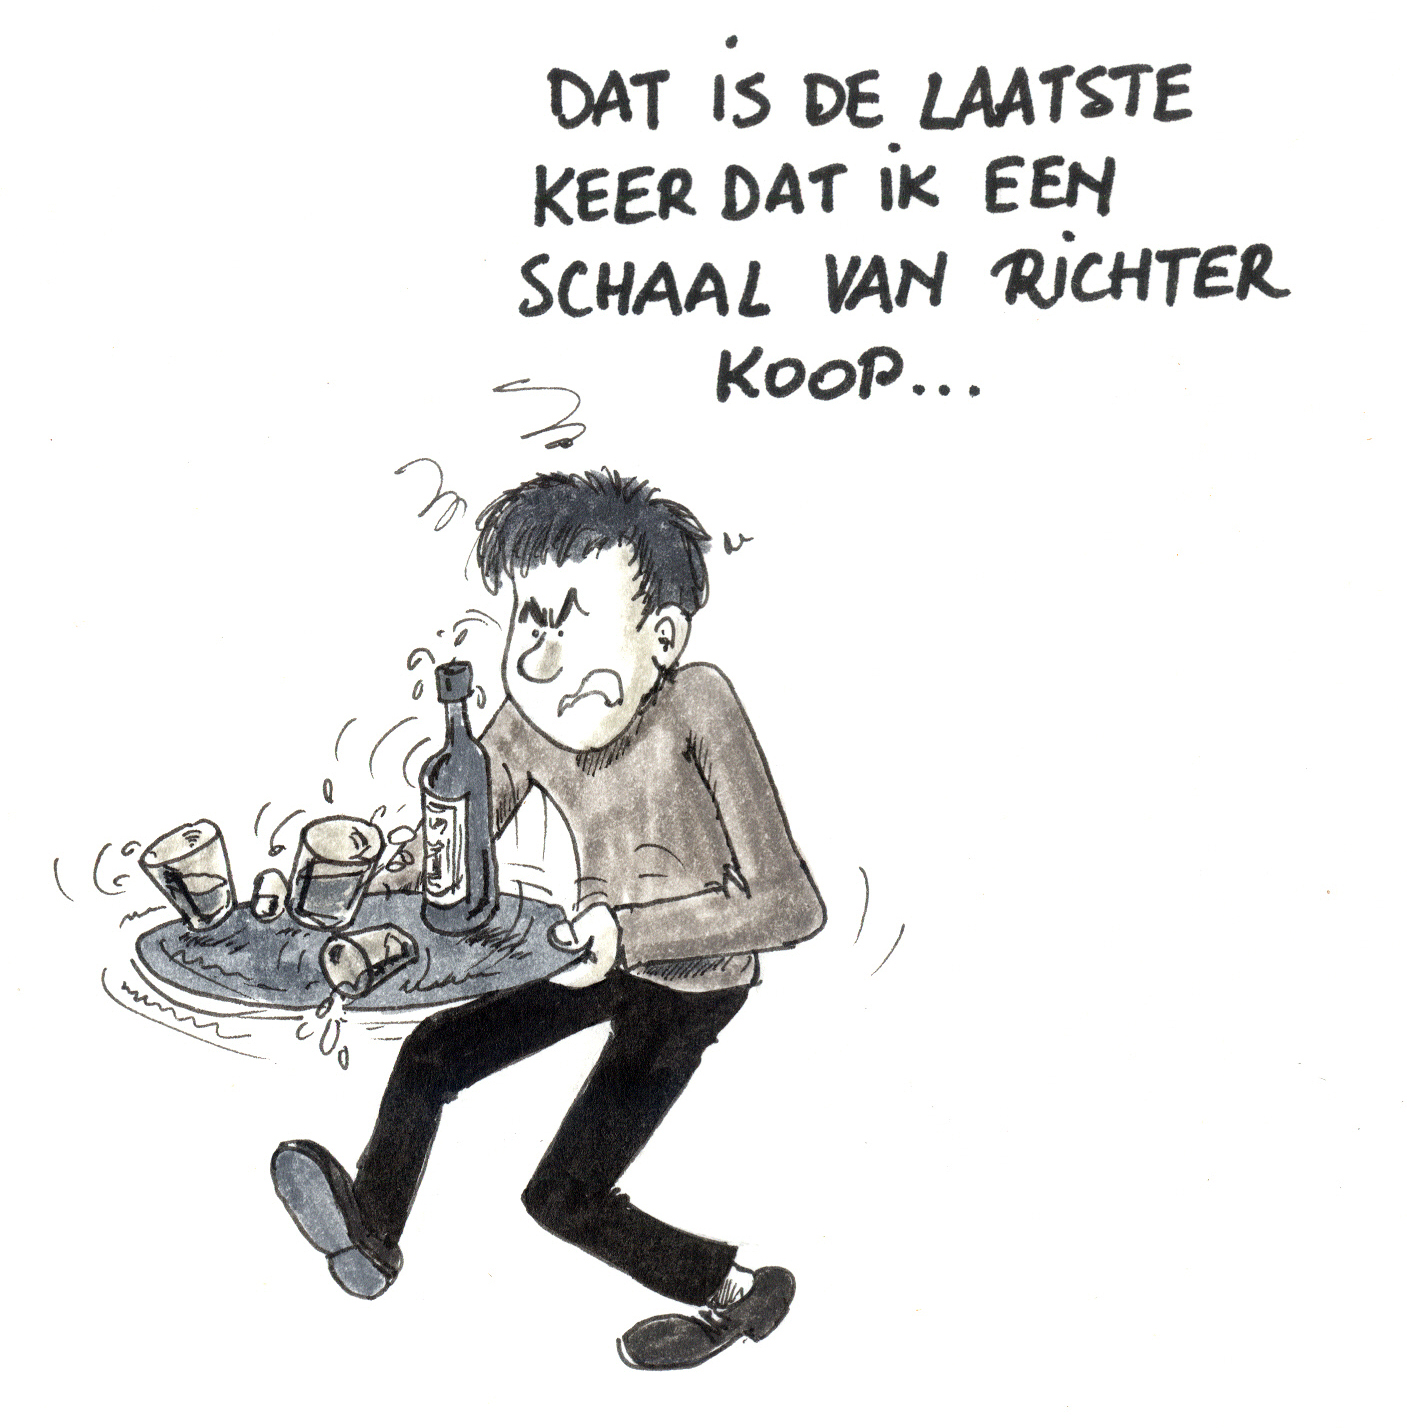
\includegraphics[width=1\linewidth]{img/richter.jpg}
\end{center}
\tussentitel{Aardbevingen}

De schaal van Richter is een logaritmische schaal die de magnitude van een aardbeving aangeeft. Het is een maat voor de energie die bij een aardbeving vrijkomt. De energie kun je vergelijken met de prikkel, de magnitude met de waarneming. De onderstaande formule geeft het verband tussen de magnitude $n$ en de vrijgekomen energie $E$, uitgedrukt in J. 
\[ n={\frac {2}{3}}\log \left({\frac {E}{2}}\right)-3\]
Een lichte aardbeving heeft een waarde van 1 tot 4, een matig zware gaat van 4 tot 6 en een zware heeft een magnitude groter dan 6. De krachtigste aardbeving ooit op aarde waargenomen had een waarde van 9,5 op de Schaal van Richter.
De hoeveelheid energie die vrijkomt bij een aardbeving wordt achteraf berekend met behulp van de bovenstaande formule.



\subsection{Audiogrammen}
Een audiogram geeft weer hoe goed of slecht je hoort en geeft het resultaat van een gehoortest weer. Bekijk goed de schaalverdeling op beide assen van figuur \ref{fig:Gehoorverlies}.
Op de horizontale as staat de frequentie die de toonhoogte bepaalt. Iemand met een gezond gehoor kan frequenties waarnemen tussen 20\,Hz en 20\,kHz. Dit is een zeer groot bereik dat je met een gewone lineaire schaal niet overzichtelijk kunt weergeven. Daarom gebruikt men hier machten van 2. Tussen twee streepjes wordt de waarde met 2 vermenigvuldigd. Opeenvolgende getallen hebben een constante verhouding. Om een bepaalde frequentie $f$ op deze schaal te zetten, neem je de $\log_{2}f$. 125\,Hz is een hele lage toon. Als je van links naar rechts door het audiogram loopt wordt de frequentie steeds hoger, net als wanneer je op het klavier van een piano van links naar rechts gaat. Het gebied met de voor spraak belangrijkste tonen ligt tussen 500 en 4000 Hz.  

Op de verticale as staat het gehoorverlies in dB. Bij elk streepje neemt de waarde met 10 toe. De schaal is lineair omdat de grootheid $L$ zelf logaritmisch is! De positieve kant van de as wijst naar onder, we meten immers een gehoorverlies. 

Je hebt waarschijnlijk ook opgemerkt dat links en rechts verwisseld zijn. Dit heeft alles te maken met het afnemen van de test: de audioloog zit tegenover de testpersoon en het rechteroor bevindt zich voor haar/hem aan de linkerkant!

\end{multicols}
\begin{figure}[H]
\begin{center}
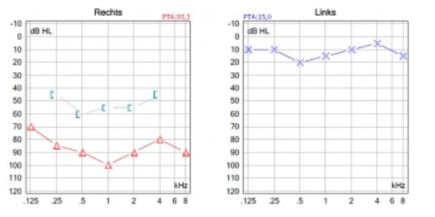
\includegraphics[width=0.6\linewidth]{img/gehoorverlies.JPG}
\captionof{figure}{Audiogram van een persoon met gehoorverlies}
\label{fig:Gehoorverlies}
\end{center}
\end{figure}
\begin{multicols}{2}
\newpage

Bij elke zuivere toon met een bepaalde frequentie of toonhoogte die in de test wordt aangeboden, past een geluidsniveau waarbij we deze toon nog net kunnen horen. Dit wordt de gehoordrempel genoemd. Per oor worden er meestal 7 toonhoogtes getest zodat er 7 gehoordrempels bepaald worden. Door deze drempels wordt een gebroken lijn getrokken die de gehoorcurve geeft. 

 Hoordrempels van 20 dB of minder worden als normaal beschouwd. De grootte van het gemiddelde gehoorverlies bij 500, 1000 en 2000 Hz wordt vaak gebruikt om het gehoorverlies te typeren:
\begin{itemize}
\item minder dan 20 dB: normaal gehoor
\item tussen 20 en 30 dB: licht gehoorverlies
\item tussen 30 en 60 dB: matig gehoorverlies
\item tussen 60 en 90 dB: ernstig gehoorverlies
\item meer dan 90 dB: zeer ernstig gehoorverlies
\end{itemize}

De persoon van figuur \ref{fig:Gehoorverlies} hoort normaal aan de linkerkant. Aan de rechterkant is er wel gehoorverlies. De stippellijn geeft het resultaat van een test met een beenvibrator om de beengeleiding te meten. De doorlopende lijn met driehoekjes geeft het resultaat van een test met een koptelefoon om de luchtgeleiding te meten. Dit onderscheid is belangrijk om de aard van het gehoorverlies te kunnen bepalen. Deze persoon scoort dus slecht op beide testen; hij lijdt aan gemengd hoorverlies.

Het audiogram in figuur \ref{fig:gehoorverliesbeiden} is van een persoon die links normaal hoort en rechts slecht scoort voor beide testen. Hoe hoger de frequentie, hoe slechter het wordt. 

\begin{figure}[H]
\begin{center}
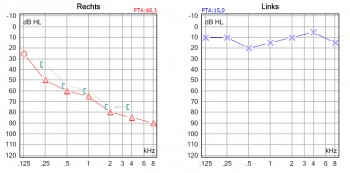
\includegraphics[width=1\linewidth]{img/gehoorverliesbeiden.jpg}
\captionof{figure}{}
\label{fig:gehoorverliesbeiden}
\end{center}
\end{figure}
\medskip
\subsection{Logaritmisch is instinctief, lineair is aangeleerd
}
Logaritmische schalen kunnen in verband gebracht worden met hoe we als baby instinctief dachten over cijfers. Bij experimenten met baby's van twee tot drie maanden oud werd de hersenactiviteit geregistreerd om te zien hoe ze veranderingen op een computerscherm waarnemen. Een verandering van acht eenden naar 16 eenden veroorzaakte activiteit in de pariëtale kwab, wat aantoont dat pasgeborenen een intuïtie van getallen hebben. De reactie van een baby is kleiner naarmate de cijfers dichter bij elkaar liggen. Maar acht en negen worden bijvoorbeeld veel dichter bij elkaar waargenomen dan één en twee. 
\end{multicols}
\begin{center}
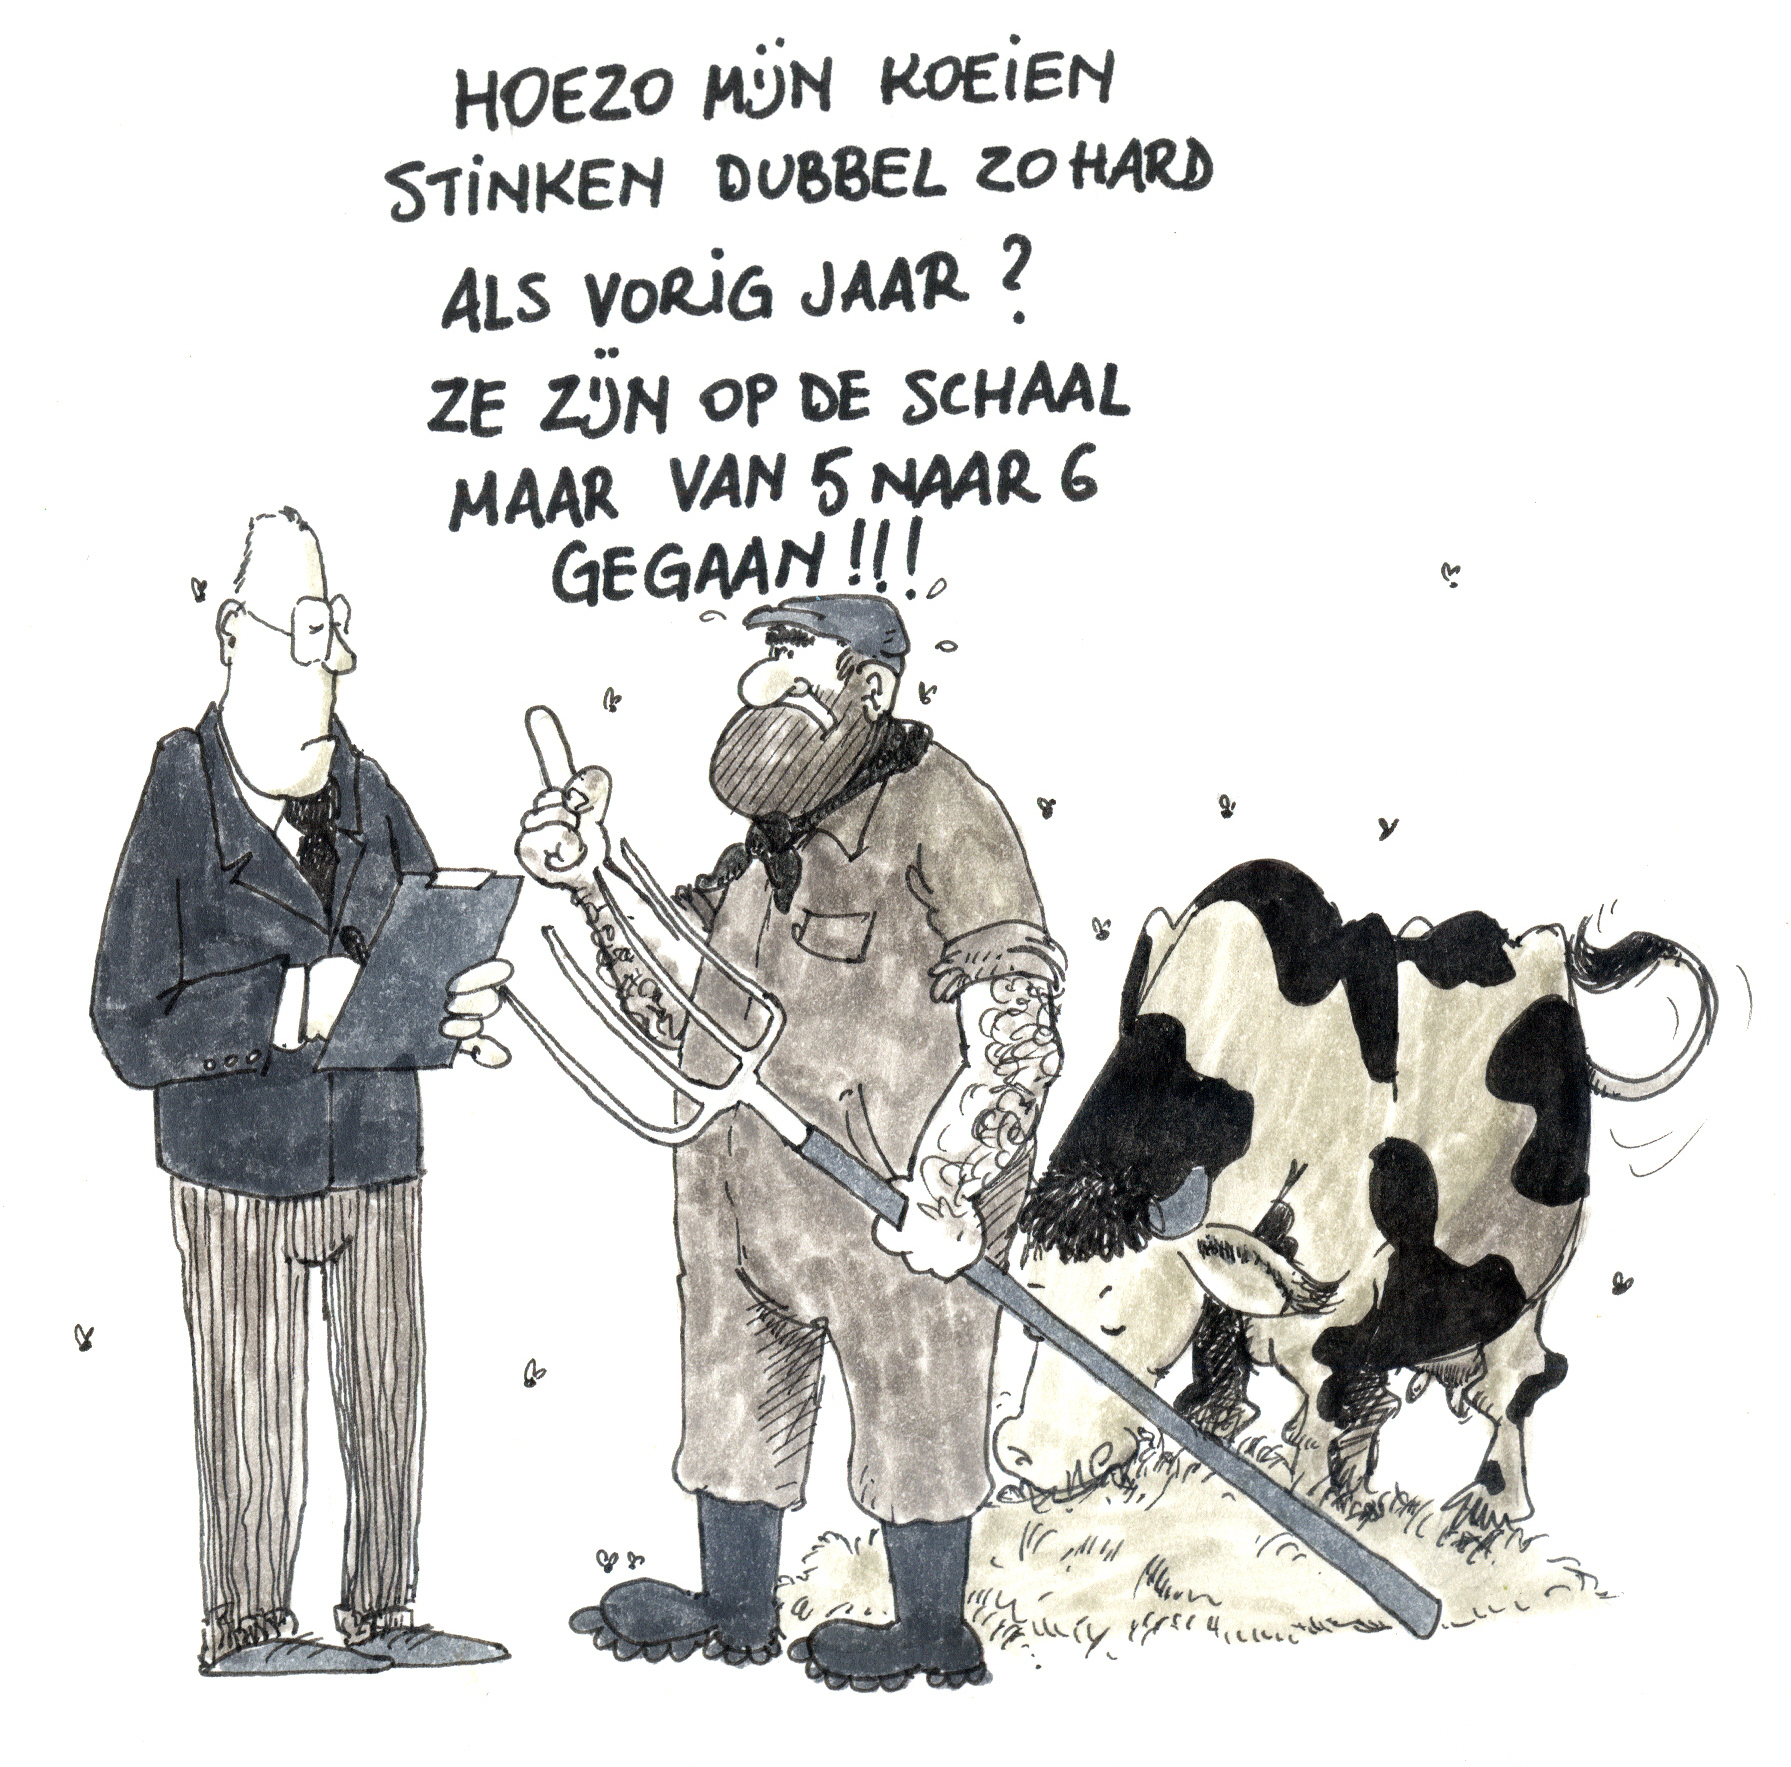
\includegraphics[width=0.52\linewidth]{img/koeienstank.jpg}
\end{center}
\begin{multicols}{2}
Het lijkt alsof ze de logaritme van het getal zien. Ze denken niet na over verschillen, ze denken na over verhoudingen.  Het is pas als ze leren tellen, en dus de getallen leren ordenen, dat ze het verschil tussen 1 en 2 even groot schatten als tussen 8 en 9. Door dit aan te leren, verdring je waar ze mee geboren zijn. 
\begin{figure}[H]
\begin{center}
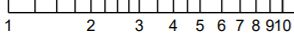
\includegraphics[width=0.5\linewidth]{img/logschaal.JPG}
\captionof{figure}{Logaritmische schaal}
\end{center}
\end{figure}

Onderzoek met mensen afkomstig uit de Amazone (Dehaene, 2008), die geen telwoorden hebben die groter zijn dan vijf, laat zien dat mensen, als ze aan hun instinct worden overgelaten, op deze manier zullen blijven denken. Als iemand één object aan de linkerkant en negen aan de rechterkant wordt getoond en wordt gevraagd: "Wat zit er in het midden?", dan zouden jij en ik vijf objecten kiezen, maar de gemiddelde Amazone kiest er drie. Wanneer we denken in termen van verhoudingen en logaritmische schalen (in plaats van verschillen en lineaire schalen), is één keer drie drie en drie keer drie is negen, dus drie is in het midden van één en negen.
Als ik echt nadenk over concrete situaties, vind ik me ook terug in het logaritmisch denken:bijvoorbeeld bij het verbeteren, het onderscheid tussen nog 25 of 26 examens te verbeteren of nog 2 of 1, het onderscheid tussen 2 of 3 snoepjes of tussen 50 en 51. De grote getallen lijken dichter bij elkaar te liggen, net zoals bij de logaritmische schaal! 


\subsection{Wet van Benford}
De Canadees-Amerikaanse wiskundige en sterrenkundige Simon Newcomb (1835-1909) merkte bij het bestuderen van grote verzamelingen data van bijvoorbeeld fysische meetresultaten, op dat er meer getallen met een 1 beginnen dan met een 2, dat er meer getallen met een 2 beginnen dan met een 3, enzovoort. Hij had dit opgemerkt omdat de eerste bladzijden van logaritmetafels er meer beduimeld en verkreukt uitzagen dan de bladzijden verderop. We gaan er van uit dat zo’n logaritmetafel enorm vaak gebruikt is en dat het gaat over enorm veel willekeurige getallen die hiermee opgezocht zijn. Intuïtief zou je denken dat alle cijfers even vaak zouden moeten voorkomen als leidend cijfer. 
Newcomb vond een eenvoudige formule waarmee de kans op het voorkomen van het leidend cijfer $d$ kon berekend worden: \\
\[P(\textrm{leidend cijfer}=d)=\log(\frac{d+1}{d}).\]
\\
Hij schreef er een artikel over maar dit was wiskundig niet genoeg uitgewerkt en bevatte ook geen statistische bewijzen.

In 1938 herontdekte Frank Benford (1883-1948) hetzelfde patroon. Hij verzamelde veel fysische constanten, metingen, wortels van getallen, populaties, rivieren, oppervlakten. De gegevens kwamen goed overeen met de formule die Newcomb een halve eeuw eerder had ontdekt. Ongeveer 30\% begon met 1, 18\% met 2 enz. Zijn analyse was een aanwijzing voor het bestaan van de wet maar ook Benford kon geen verklaring geven. De formule kreeg wel zijn naam en is verder bekend als de wet van Benford.

\tussentitel{Zelf experimenteren}
De wet van Benford kun je zelf experimenteel controleren met een eenvoudig rekenblad. Je kunt in Excel bijvoorbeeld duizend producten van 3 toevalsgetallen laten berekenen door de volgende formule in te geven en door te voeren naar 1000 cellen:\\
$=(9*ASELECT()+1)*(9*ASELECT()+1)*(9*ASELECT()+1)$.\\
Met de volgende formule laat je het leidende cijfer berekenen:\\ $=LINKS(A1;1)$\\
Met de laatste formule kun je de relatieve frequentie berekenen van elk cijfer, bv. voor 1:\\
$=AANTAL.ALS(B$1:B$1000;1)/1000 $

Je kunt het rekenblad de berekening een aantal keer laten uitvoeren, je kunt het aantal getallen nog opvoeren. De getallen van de tweede kolom wijken weinig af van de getallen in de derde kolom.
Je kunt je afvragen waarom een product van drie getallen nodig is. Verbetert het als je het product neemt van 4 getallen? Wat gebeurt er als je het product van 2 getallen laat berekenen? Dit werkt niet omdat de uniforme toevalsgenerator van Excel nog te prominent aanwezig is. Eventueel kun je ook nog onderzoeken of de Fibonaccigetallen voldoen aan de wet van Benford. 
\end{multicols}
\begin{figure}[H]
\begin{center}
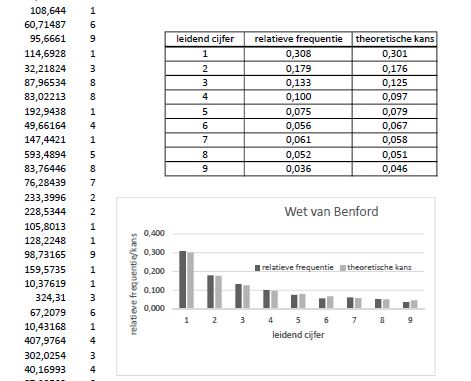
\includegraphics[width=1\linewidth]{img/excelbenford.JPG}
\captionof{figure}{Wet van Benford met rekenblad}
\end{center}
\end{figure}
\begin{multicols}{2}

\tussentitel{De verklaring}
De eerste stap naar een verklaring van deze wet is gezet door Roger Pinkman in 1961. Zijn argument was het volgende: veronderstel dat de wet van de leidende cijferfrequenties echt is, dan moet ze universeel zijn. Als je iets meet in km of in mijl, prijzen uitdrukt in dollar of ponden, de verhouding van de leidende cijfers moet gelijk blijven. Of anders gezegd, de verdeling van de leidende  cijfers moet `schaalinvariant' zijn.

Wat betekent dit?
We gaan uit van een grote verzameling numerieke data $D$, bijvoorbeeld de lengtes van alle rivieren in de wereld. Als we elk getal van de verzameling $D$ bijvoorbeeld met 2 vermenigvuldigen, ontstaat een verzameling $D'$. Een getal in $D$ dat met een 1 begint, zal na vermenigvuldiging met 2, een getal in $D'$ opleveren dat begint met 2 of 3. Een getal uit $D$ dat begint met een 2, zal in $D'$ overgaan in een getal dat begint met 4 of 5. Maar als het leidend cijfer van getallen in $D$  5 of 6 of 7 of 8 of 9 is, zal dat steeds een getal met leidend cijfer 1 opbrengen in $D'$.
\begin{center}
\begin{tabular}{ |l| l| }
\hline
  Leidend cijfer &Leidend cijfer \\
  voor transformatie&na transformatie\\ \hline
  1 &2 of 3 \\ \hline
  2 & 4 of 5 \\ \hline
 3 &6 of 7 \\ \hline
  4 & 8 of 9 \\ \hline
 5,6,7,8,9 &1\\ \hline
\end{tabular}
\end{center}

Als we veronderstellen dat de leidende cijfers in elke numerieke dataverzameling uniform verdeeld zijn, dan is de kans dat een getal begint met $d$ gelijk aan $\frac{1}{9}$.

Een eenvoudige transformatie als hierboven laat zien dat deze veronderstelling niet juist kan zijn. De kansverdeling van het leidende cijfer moet in $D'$ hetzelfde zijn als in $D$, en dat is onmogelijk bij een uniforme kansverdeling. 
De vraag is dan aan welke universele kansverdeling het leidende cijfer moet voldoen en waarom.

In 1995 publiceert Theodore P. Hill een artikel waarin hij bewijst dat de logaritmische distributie voor het leidende cijfer de enig mogelijke distributie is. Hij bewijst dus dat als schaalinvariantie optreedt, de wet van Benford geldt. Wie geïnteresseerd is in een bewijs, verwijzen we naar Walthoe (1999).     

\tussentitel{Toepassingen}
Kan je in het vervolg beter rekening houden met de wet van van Benford als je een lottoformulier invult? Neen, de wet van Benford geldt niet in elke willekeurige dataset. Hoe willekeuriger en hoe groter het bereik van de grootte van de getallen zijn, hoe dichter de kansverdeling bij de wet van Benford ligt. De getallen van de loterij zijn volledig ad random, dat wil zeggen dat elke loterijnummer evenveel kans heeft om voor te komen. Het leidende cijfer zal daarom net zoveel voorkomen als dat er loterijnummers zijn die beginnen met dat cijfer. 

Als je de olympische looptijden van 400 m bekijkt, uitgedrukt in s, zullen die ook niet dikwijls met een 1 beginnen. Ze liggen bij elkaar in de buurt.
De wet van Benford heeft getallen nodig die niet totaal ad random zijn maar ook niet te dicht bijeen liggen of normaal verdeeld zijn, eerder iets tussenin.
De gegevens kunnen erg gespreid zijn en moeten het resultaat van verschillende processen, met verschillende invloeden zijn. Bijvoorbeeld de bevolkingsaantallen in steden.

Waar is dit nu goed voor?
De wet van Benford wordt sinds de jaren 90 nuttig ingezet voor fraudedetectie bij grote hoeveelheden financiële data. In gevallen dat de wet van Benford zou moeten of kunnen optreden, maar dit niet doet, kan dit duiden op fraude. Toch moet er goed worden opgelet, omdat niet elke dataset hoeft te voldoen aan de wet van Benford! 
\end{multicols}


\stopcontents[mainsections]			        % altijd laten staan, opsomming in inhoudstafel enkel tot loep beperken


% bronnen toevoegen
\begin{bronnen}

\item Baierlein M., e.a. (1997). \emph{Anschauliche Analysis 2}. R. Oldenbourg Verlag GmbH, München,  ISBN 3-486-02291-1

\item Blasjo (2016). How to find the logarithm of any number using nothing but a piece of string. \emph{The College Mathematics Journal 47/2}, 95-100. Besproken in Uitwiskeling 34/4.

\item Brüel \& Kjaer (2002). \emph{Sound \& Vibration Measurement A/S}

\item Clark, K., Montelle, C. (2011). Logarithms: The Early History of a Familiar Function, \emph{Convergence, January 2011}. 

https://www.maa.org/press/periodicals/convergence/logarithms-the-early-history-of-a-familiar-function-john-napier-introduces-logarithms

\item Daems, J. (2019). Wortels van de wiskunde: logaritmen. \emph{Euclides 95/5}, 12-15.

\item De Bock, D., Eggermont, H., Roelens, M. (1990). \emph{Context: exponentiële en logaritmische functies}, Deurne: Plantyn. 

\item De Decker, E. (1626). \emph{Nieuwe telkonst inhoudende de logarithmi van de ghetallen beginnende van 1 tot 10000 ghemaeckt van Henrico Briggio professor van de Geometrie tot Ocxfort.}

\url{https://books.google.be/books?id=fqi_nclcw8gC&lpg=PA13&ots=3QRIBRGTAe&dq=\\"meetkonstighe\%20exempelen"}.

\item Dehaene S., e.a.(2008). \emph{Log or Linear? Distinct Intuitions of the Number Scale in Western and Amazonian Indigene}. Culture’, Science, 30 mei 2008.

https://pdfs.semanticscholar.org/5d84/b5124ec64c56c8f812116ce009dc8d79b736.pdf.

\item Eggermont, H., Vanlommel, E. (2012). Priemgetallen. \emph{Uitwiskeling 28/3}.

\item Resnikoff, H.L., Wells, R.O. (1973). \emph{Mathematics in civilization}. New York: Dover Publications.

\item Roels, J. e.a. (1990). \emph{Wiskunde vanuit toepassingen. Functies en matrices als modellen}. Leuven: Aggregatie HSO Wiskunde K.U.Leuven.

\item Schons, N.J., De Cock, C. (z.d.). \emph{Logaritmentafels in vijf decimalen en bijtafels}. Brussel/Namen: De Procure.

\item Stifel, M. (1544). \emph{Arithmetica Integra}. 

\item Swets, F. e. a. (Eds.) (1995). \emph{Learn from the Masters.} Washington: The Mathematical Association of America.

\item Trompler, S. (2002). \emph{ L'histoire des logaritmes.} Unité de Recherche sur l’Enseignement des Mathématiques, Brussel: Université Libre de Bruxelles.

\item van der Salm, S. (2002). \emph{Rekenonderwijs op de liniaal.} \url{http://www.rekeninstrumenten.nl/MIR/MIR%20Articles/Mir32%2023%20rekenonderwijs.pdf}

\item van Poelje, O. (2014). \emph{Logaritmen en rekenlinialen - 400 jaar werktuig in beroep en onderwijs}.\\ \url{http://www.fisme.science.uu.nl/nwd/nwd2014/handouts/handouts.html}

\item Walthoe J. \emph{Looking out for number one.}
\url{https://plus.maths.org/content/looking-out-number-one}

\item Wepster, S. (2017). Logaritmen: hoe en waarom. \emph{Pythagoras 57/1}, 12-15.

\item Wolf, R. P. (last update 2019) \emph{Collection of Slide Rule replicas} \url{http://www.sliderules.org/} (veel apps voor rekenlinialen)

\item \url{http://www.fi.uu.nl/wiskrant/artikelen/282/282december_salm.pdf} 

\item \url{https://static.scientificamerican.com/sciam/assets/media/pdf/Slide_rule.pdf} (Uitknipversie rekenlineaal.)

\item \url{https://natuurkundeuitgelegd.nl/fotonpdf/FotonMenselijkLichaamHAVO.pdf}

\item \url{http://www.fi.uu.nl/wiskrant/artikelen/282/282december_salm.pdf} 

\item \url{https://neus-keel-oor.be/nl/nko/oor/onderzoeken/audiogram/}

\item \url{https://www.oorcheck.nl/gehoorschade/hoe-ontstaat-schade/wat-te-hard/} 

\item \url{http://www.natuurinformatie.nl/ndb.mcp/natuurdatabase.nl/i000332.html}

\end{bronnen}

